\documentclass[12pt,a4paper]{ufpr}

% \usepackage[portuges,brazil]{babel}
% \usepackage[portuguese,brazil]{babel}

\usepackage[brazil]{babel}
\usepackage[latin1]{inputenc}
\usepackage{amssymb,amsmath}
\usepackage{epsfig}
\usepackage{multirow}

\usepackage{lmodern} % load a font with all the characters

%\usepackage[portugues,ruled,lined,titlenotnumbered,figure]{algorithm2e}
%\usepackage{algorithmic}
\usepackage[named]{algo}


%\usepackage{isolatin1}
\usepackage{amssymb}
\usepackage{subfigure}
\usepackage{graphicx}
\usepackage{caption}
\usepackage{setspace}
\usepackage{ps-macros}
% \usepackage{psfig}

\usepackage{listings}
\usepackage{color}

\definecolor{mygreen}{rgb}{0,0.6,0}
\definecolor{mygray}{rgb}{0.5,0.5,0.5}
\definecolor{mymauve}{rgb}{0.58,0,0.82}
\definecolor{mybckg}{rgb}{0.95,0.95,0.95}

\setcounter{secnumdepth}{2}    % n - numero de niveis de subsubsection numeradas
\setcounter{tocdepth}{1}       % coloca ate o nivel n no sumario

\title{Simula��o do Protocolo de Roteamento OSPF com NS-3}
\author{Mozart Pistori Tomazetti}
\advisortitle{Orientador} % ou Orientador
\advisorname{Prof. Dr. Elias P. Duarte Jr.}
\advisorplace{Departamento de Inform�tica, UFPR}  % departamento, instituicao
\city{Curitiba}
\year{2013}

\banca        % nao insira o nome do orientador, ja eh feito automaticamente
{Prof. Dr. Nome exmplo}{Instituto exemplo, UE}
{Prof. Dr. Nome exmplo}{Departamento de Inform�tica, UFPR}
{}{} % se nao houver deixe em branco {}{}
{}{}    % se houver um quarto membro na banca, inserir nome e instituicao

\defesa{21 de dezembro de 2013} % dia em que foi realizada a defesa da dissertacao


\begin{document}

%\makecapaproposta             % cria capa para proposta%
\makecapadissertacao           % cria capa para dissertacao de mestrado %
%\makerosto                     % cria folha de rosto para versao final da UFPR %
%\maketermo                     % cria folha com o termo de aprovacao da dissertacao%

%\singlespacing           % espacamento 1 - capa UFPR%
%\onehalfspacing          % espacamento 1/2 %
\doublespacing            % espacamento 2 - UFPR %

\pagestyle{headings}
\pagenumbering{roman}

%\chapter*{Agradecimentos}
%\input{agradecimentos.tex}          % possiu somente o texto

\tableofcontents

%\listoffigures         % se houver mais do que 3 figuras
%\addcontentsline{toc}{chapter}{\MakeUppercase{Lista de Figuras}}
%\newpage

%\listoftables        % se houver mais do que 3 tabelas
%\addcontentsline{toc}{chapter}{\MakeUppercase{Lista de Tabelas}}
%\newpage

\chapter*{Resumo}
\addcontentsline{toc}{chapter}{\MakeUppercase{Resumo}}
%Texto do resumo....
	Nos últimos anos, tem-se observado um grande crescimento na utilização de sistemas robóticos no dia a dia.
	Cada vez mais pesquisadores em robótica têm se concentrado no desenvolvimento de robôs móveis, fazendo com que os
	 robôs possam se mover e interagir com o ambiente de forma autônoma, 
	o que abre um vasto campo de novas aplicações e, consequentemente, muitos desafios, como:  localização, construção de mapas e o problema
	de auto localização e construção 
  de mapas de ambiente simultâneos(\textit{Simultaneous Localization and Map Building - SLAM}). 
		
    Este trabalho propõe um sistema de localização para robôs móveis, 
    baseado no método empírico sugerido no artigo \cite{wifiRadar},
    que provê a localização de um terminal móvel em um ambiente \textit{indoor}. 
    O método é baseado na força do 
    sinal recebido(\textit{Received Signal Strength} - RSS), que é muito explorada em
    em técnicas de localização em uma rede de sensores sem fio pela fácil aplicabilidade. Serão apresentadas também, outras 
    técnicas utilizadas na localização em uma rede de sensores sem fio.
  
	Todo o sistema foi desenvolvido na plataforma Android, pela sua fácil incorporação à robótica devido ao 
	grande quantidade de sensores suportados. Serão brevemente comentadas
	algumas características deste sistema operacional e de uma aplicação Android.
   
   Os resultados obtidos pelo sistema proposto mostram que:
      \begin{itemize}
      \item 22,8\% das estimativas possuem precisão de 1 metro ou menos.
      \item 77,1\% das estimativas possuem precisão de 3 metros ou menos.
      \item 91,4 \% das estimativas possuem precisão de 5 metros ou menos.
     \end{itemize}
	
\textbf{Palavras-chave:} RSS, Localização, RSS fingerprint, Robós Móveis, Android, WSNs.           % somente o texto
\newpage

%\chapter*{Abstract}
%\addcontentsline{toc}{chapter}{\MakeUppercase{Abstract}}
%  
  \textbf{Keywords:} MEAN, Javascript, Node.js, Angular.js, MongoDB, Express.js, Scalability.        % somente o texto
%\newpage


\pagenumbering{arabic}

\chapter{Introdu\c{c}\~ao}
\label{Introducao}

%Quando ocorre uma falha em uma rede na qual os roteadores estam rodando o protocolo \textit{OSPF} informa��o deixa de ser transmitida. Os pacotes devem esperar o \textit{OSPF} encontrar um novo caminho para que possam ser novamente transmitidos. Sendo assim, a comunica��o entre alguns roteadores da rede fica inativa. Como o \textit{OSPF} faz parte dos protocolos utilizados na Internet � essencial que este intervalo, no qual a comunica��o fica inativa, seja o menor poss�vel. Durante este intervalo os roteadores pertencentes a rede s�o informados que occoreu uma falha e devem encontrar um novo caminho. O novo caminho a ser encontrado deve ser m�nimo. Uma solu��o para n�o interromper a comunica��o na rede durante uma falha seria os roteadores utilizarem um caminho alternativo at� que seja encontrado um novo caminho. O caminho alternativo n�o precisa ser m�nimo, pois ele � um caminho tempor�rio com a fun��o de manter a comunica��o da rede at� todos os roteadores sejam informados de uma falha e encontrem um novo caminho m�nimo. Entretanto � preciso analisar esta solu��o, verificar se ela � vi�vel. Para isso � preciso implementar o novo algoritmo e comparar sua efic�cia em rela��o ao \textit{OSPF}.

%O restante deste trabalho est� organizado da seguinte maneira. O cap�tulo 2 descreve o funcionamento dos protocolos semelhantes ao \textit{OSPF}. Al�m disso, s�o analisadas as vantagens e os detalhes do \textit{OSPF}; como o \textit{OSPF} encontra o caminho m�nimo entre os roteadores da redes e como acontece a troca de informa��es de controle entre os roteadores. O cap�tulo 3 descreve passo a passo como instalar e configurar o simulador \textit{NS-3} para que seja poss�vel realizar simula��es do \textit{OSPF}. O cap�tulo 4 mostra como utilizar o \textit{NS-3}; como criar a topologia da rede e configurar cada roteador para utilizar o protocolo \textit{OSPF}. Al�m disso s�o analisados os resultados obtidos nas simula��es.

%O NS-3 permite executar a simula��o de diversos protocolos. Um destes protocolos � o OSPF, que contribui para o roteamento de pacotes na Internet. � poss�vel utilizar o NS-3 para observar o funcionamento do OSPF. Entretanto, nas simula��es que ocorre uma falha de enlace todos os pacotes que passam por este enlace n�o chegam aos seus destinos. Esse comportamento se mant�m por tempo indefinido. Sendo assim, � poss�vel perceber que a implementa��o do protocolo OSPF, nativa do NS-3, � muito limitada. Uma vez que, quando um enlace falha, os roteadores da rede deveriam calcular novos caminhos. Por�m isso n�o acontece nas simula��es. Deste modo, o m�dulo do NS-3 chamado DCE passa a ser uma alternativa para simular o protocolo OSPF. O DCE possui a implementa��o do protocolo OSPF feita pela \textit{Quagga Routing Suite}. Ao utilizar o DCE, quando um enlace falha os roteadores encontram um novo caminho m�nimo e os pacotes passam a utilizar este caminho.

A Internet � dividida em conjuntos de roteadores. Cada conjunto de roteadores est� sob o controle de uma �nica entidade administrativa. Dentro destes conjuntos os roteadores trocam informa��es atrav�s do protocolo de roteamento interno. Al�m disso, os protocolos de roteamento s�o tipicamente classificados em dois tipos: vetor de dist�ncia e estado de enlace. O \textit{Open Shortest Pah First} (OSPF) \cite{Reference6} � um protocolos de roteamento interno do tipo estado de enlace. O OSPF utiliza descri��es do estado dos enlaces da rede para criar um representa��o da topologia da rede na forma de um grafo. A partir dessa representa��o, os roteadores utilizam o algoritmo de Dijkstra \cite{Reference10} para calcular o caminho m�nimo de uma origem para cada destino da rede. A cria��o e manuten��o desta representa��o da topologia � feita, principalmente, por tr�s subprotocolos que juntos formam o OSPF. O protocolo \textit{Hello} que tem o objetivo de verificar o estado dos enlaces e eleger um roteador designado e um roteador reserva. Quando dois roteadores estabelecem conectividade bidirecional, o protocolo \textit{Exchange} � repons�vel pela sincroniza��o da representa��o local da topologia da rede. Al�m disso, o protocolo \textit{Flooding} � repons�vel por informar a todos os roteadores quando ocorre uma falha na rede.

 O \textit{Network Simulator 3} (NS-3) \cite{Reference12} � um simulador de eventos discretos, voltado principalmente para simula��o de redes de computadores. O simulador NS-3 � um software livre dispon�vel publicamente. O NS-3 � constru�do como um sistema de bibliotecas de \textit{software}. Estas bibliotecas s�o escritas na linguagem C++.
 
Este trabalho descreve como simular o OSPF no NS-3. Inicialmente � avaliado o uso do \textit{Global Route Manager} que � respons�vel por preencher as tabelas de roteamento do roteadores. Entretanto, o \textit{Global Route Manager} n�o implementa um protocolo de roteamento. Uma vez que, ele somente calcula caminhos est�ticos, pois as tabelas de roteamento s�o preenchidas antes de iniciar o tr�fego de pacotes na rede. Portanto, n�o s�o utilizados pacotes de controle e quando ocorre uma falha na rede os rotedores n�o s�o informados. Sendo assim, um m�dulo do NS-3 chamado \textit{Direct Code Execution} (DCE) passa a ser uma alternativa para simular o protocolo OSPF. O DCE permite executar aplica��es reais dentro do NS-3 e uma destas aplica��es a implementa��o do protocolo OSPF feita pela \textit{Quagga Routing Suite} \cite{Reference14}. O Quagga fornece implementa��es de protocolos de roteamento para as plataformas Unix. Ao executar as simula��es � poss�vel observar o comportamento do OSPF implementado no m�dulo DCE. O funcionamento da implementa��o do DCE � semelhante ao da implementa��o nativa do NS-3. Entretanto, � poss�vel notar a diferen�a entre as duas implementa��es nas simula��es em que ocorrem falhas na rede. Na implementa��o do NS-3 quando ocorre um falha de enlace, todos os pacotes que utilizavam o caminho afetado s�o perdidos. No OSPF do DCE somente alguns pacotes s�o perdidos, pois os roteadores percebem a falha do enlace e encontram um novo caminho m�nimo.

Entretanto, o DCE n�o � nativo do NS-3 e isso adiciona complexidade ao procedimento de simular o OSPF. Caso o NS-3 seja instalado de acordo com sua documenta��o, o m�dulo DCE n�o � instalado e � necess�rio refazer a instala��o para permitir o uso do DCE. Al�m disso, a maneira de configurar a simula��o passa por diversas mudan�as quando � utilizado o DCE e grande parte do conhecimento adquirido ao utilizar o NS-3 se torna obsoleto. De fato, usar o DCE implica em trabalhar com a pr�pria implementa��o do protocolo no sistema operacional, o que elimina a vantagem da simula��o, na medida em que m�ltiplos detalhes devem ser considerados mesmo para testes simples. Al�m disso, a documenta��o do DCE, especialmente a parte relacionada ao OSPF, � insuficiente e incompleta.

O restante deste trabalho est� organizado da seguinte maneira. O cap�tulo 2 descreve as caracter�sticas do protocolo OSPF. O cap�tulo 3 descreve os procedimentos necess�rios para instalar e configurar o NS-3 para simular o OSPF. O cap�tulo 4 descreve execu��o de simula��es do protocolo OSPF no NS-3 e o uso do DCE. Finalmente, o cap�tulo 5 traz as conclus�es.

\chapter{O Protocolo OSPF}
\label{O Protocolo OSPF}

Este cap�tulo descreve o protocolo de roteamento da Internet \textit{Open Shortest Path First} (OSPF). Antes, uma vis�o geral do roteamento na Internet apresenta os conceitos de sistemas aut�nomos e protocolos de roteamento interno e externo. Em seguida, s�o descritas as tecnologias de roteamento denominadas vetor de dist�ncia e estado de enlace. O cap�tulo termina com uma descri��o detalhada do protocolo OSPF.

\lstset{
  breakatwhitespace=false,         % sets if automatic breaks should only happen at whitespace
  basicstyle=\footnotesize,
  breaklines=true,                 % sets automatic line breaking
  keepspaces=true,                 % keeps spaces in text, useful for keeping indentation of code (possibly needs columns=flexible)
  columns=flexible,
  literate=
  {�}{{\'a}}1 {�}{{\'e}}1 {�}{{\'i}}1 {�}{{\'o}}1 {�}{{\'u}}1
  {�}{{\'A}}1 {�}{{\'E}}1 {�}{{\'I}}1 {�}{{\'O}}1 {�}{{\'U}}1
  {�}{{\`a}}1 {�}{{\'e}}1 {�}{{\`i}}1 {�}{{\`o}}1 {�}{{\`u}}1
  {�}{{\`A}}1 {�}{{\'E}}1 {�}{{\`I}}1 {�}{{\`O}}1 {�}{{\`U}}1
  {�}{{\"a}}1 {�}{{\"e}}1 {�}{{\"i}}1 {�}{{\"o}}1 {�}{{\"u}}1
  {�}{{\"A}}1 {�}{{\"E}}1 {�}{{\"I}}1 {�}{{\"O}}1 {�}{{\"U}}1
  {�}{{\^a}}1 {�}{{\^e}}1 {�}{{\^i}}1 {�}{{\^o}}1 {�}{{\^u}}1
  {�}{{\^A}}1 {�}{{\^E}}1 {�}{{\^I}}1 {�}{{\^O}}1 {�}{{\^U}}1
  {�}{{\oe}}1 {�}{{\OE}}1 {�}{{\ae}}1 {�}{{\AE}}1 {�}{{\ss}}1
  {�}{{\c c}}1 {�}{{\c C}}1 {�}{{\o}}1 {�}{{\r a}}1 {�}{{\r A}}1
  {�}{{\EUR}}1 {�}{{\pounds}}1,
  %basicstyle=\ttfamily
}

%----------------------------------------------------------------------------------------
%	SECTION 1
%----------------------------------------------------------------------------------------
\section{Roteamento na Internet}

A Internet � organizada em regi�es chamadas sistemas aut�nomos \cite{Reference1}. Cada sistema aut�nomo consiste em um conjunto de roteadores sob o controle de uma �nica entidade administrativa. Dentro de um sistema aut�nomo os roteadores trocam informa��es atrav�s do protocolo de roteamento interno; para trocar informa��es entre sistemas aut�nomos � utilizado o protocolo de roteamento externo.

Todos os roteadores que pertencem a um �nico sistema aut�nomo devem permanecer conectados entre si \cite{Reference3}. Isto significa que os roteadores devem trocar informa��es para manter a conectividade do sistema aut�nomo. Um protocolo de roteamento interno � usado para configurar e manter as tabelas de roteamento dentro dos sistemas aut�nomos \cite{Reference4}. Segundo Comer \cite{Reference2}, os roteadores pertencentes ao mesmo sistema aut�nomo se comunicam periodicamente entre si a fim de trocar informa��es de roteamento. Existem diversos protocolos para uso dentro de um sistema aut�nomo. Parte do motivo para a diversidade vem das v�rias topologias e tecnologias em uso. Como resultado, v�rios protocolos se tornaram populares. Como n�o existe um padr�o �nico, o termo \textit{Interior Gateway Protocol} (IGP) � utilizado como uma descri��o gen�rica para qualquer protocolo que os roteadores internos usam quando trocam informa��es de roteamento. Um �nico roteador pode utilizar dois protocolos de roteamento diferentes simultaneamente, um para comunica��o fora de seu sistema aut�nomo e outro para comunica��o dentro de seu sistema aut�nomo.

De acordo com Huitema \cite{Reference3}, dividir a Internet em v�rios sistemas aut�nomos visa reduzir a sobrecarga de roteamento e facilitar a gest�o da rede. As tabelas de roteamento de um sistema aut�nomo devem permitir que pacotes sejam enviados para todos os poss�veis destinos da Internet. As tabelas de roteamento s�o mantidas pelos protocolos de roteamento. Por�m as mensagens do protocolo de roteamento interno s� transitam dentro do sistema aut�nomo. Os roteadores devem obter informa��es sobre redes externas. Para obter informa��es sobre redes externas � necess�rio realizar a troca de mensagens atrav�s de roteadores externos, que s�o pontos de entrada em sistemas aut�nomos adjacentes. A fun��o do protocolo de roteamento externo � realizar a troca de informa��es de acessibilidade. Esta informa��o consiste de um conjunto de redes alcan��veis. Quando um roteador externo recebe informa��es de um outro roteador externo, ele utiliza o protocolo de roteamento interno para distribuir estas informa��es dentro do sistema aut�nomo.

Kurose e Ross \cite{Reference4} ressaltam algumas das diferen�as entre o protocolo de roteamento interno e externo. Os protocolos de roteamento externo t�m como prioridade transmitir pol�ticas espec�ficas de roteamento. Como o roteamento externo � orientado a pol�ticas, n�o h� prefer�ncia ou custos associados aos caminhos. Contudo, nos protocolos de roteamento interno as preocupa��es pol�ticas podem ser ignoradas. Deste modo, os algoritmos de roteamento interno priorizam calcular, de maneira r�pida, os melhores caminhos.

Segundo Kurose e Ross \cite{Reference4}, tr�s protocolos de roteamento t�m sido usados para roteamento dentro de sistemas aut�nomos na Internet: o \textit{Routing Information Protocol} (RIP), o \textit{Open Shortest Pah First} (OSPF) e o \textit{Enhanced Interior Gateway Routing Protocol} (EIGRP), propriet�rio da Cisco. A vers�o 2 do protocolo de roteamento interno RIP est� definida na RFC 2453 \cite{Reference5}. A vers�o 2 do protocolo de roteamento interno OSPF est� definida na RFC 2328 \cite{Reference6}. O protocolo OSPF possui uma nova vers�o dedicada ao IPv6 que est� definida na RFC 5340 \cite{Reference15}. Atualmente o protocolo utilizado para roteamento entre sistemas aut�nomos � o \textit{Border Gateway Protocol} (BGP). A vers�o 4 do protocolo de roteamento externo BGP est� definida na RFC 4271 \cite{Reference7}.

%A principal fun��o de um protocolo de roteamento externo � permitir que um sistema aut�nomo se comunique com outro \cite{Reference2}. Para realizar sua fun��o, o protocolo de roteamento externo, anuncia a alcan�abilidade da rede para outros sistemas aut�nomos \cite{Reference2,Reference3}. Atualmente, o �nico protocolo de roteamento externo utilizado na Internet � o \textit{Border Gateway Protocol (BGP)} \cite{Reference3}. O protocolo BGP 

%Todos os protocolos de roteamento TCP/IP t�m maneiras de descobrir, para cada endere�o IP, o pr�ximo salto para encaminhar o tr�fego de dados. Como a rede muda os protocolos de roteamento reavaliam continuamente o pr�ximo salto utilizado para acessar cada endere�o. O processo para encontrar o novo pr�ximo salto ap�s uma mudan�a na rede � chamado de converg�ncia. N�s preferimos protocolos de roteamento que encontrem o novo pr�ximo salto de maneira r�pida, isto �, protocolos com baixo tempo de converg�ncia. Entretanto conforme o tamanho e a complexidade da rede aumentam o tempo de converg�ncia tamb�m aumenta. \cite{Reference1}

%Os protocolos de roteamento interno priorizam calcular, de maneira r�pida, os melhores caminhos. No entanto, os protocolos de roteamento externo t�m como prioridade transmitir pol�ticas espec�ficas de roteamento. Normalmente a diferen�a entre as duas classes de protocolos de roteamento associa o uso da tecnologia de estado de enlace aos protocolos de roteamento interno. \cite{Reference1}

%----------------------------------------------------------------------------------------
%	SECTION 2
%----------------------------------------------------------------------------------------
\section{Classifica��o de Protocolos de Roteamento}

Os protocolos de roteamento s�o tipicamente classificados em dois tipos: vetor de dist�ncia e estado de enlace, descritos a seguir.

\subsection{Vetor de Dist�ncia}

De acordo com Kurose e Ross \cite{Reference4}, um protocolo do tipo vetor de dist�ncia � iterativo, ass�ncrono e distribu�do. � distribu�do porque cada roteador recebe informa��es de um ou mais vizinhos diretamente ligados a ele. Com as informa��es recebidas, o roteador realiza c�lculos e distribui os resultados para seus vizinhos. � iterativo porque esse processo continua at� que mais nenhuma informa��o seja trocada entre vizinhos. � ass�ncrono porque n�o requer que todos os roteadores executem determinadas opera��es em intervalos regulares. A principal estrutura de dados de um protocolo vetor de dist�ncia � a tabela de dist�ncias. Cada roteador mant�m uma tabela de dist�ncias. A tabela de dist�ncias cont�m uma linha para cada destino na rede e uma coluna para cada um de seus vizinhos adjacentes. Cada c�lula da tabela de dist�ncias indica o custo do caminho at� o destino correspondente (linha) atrav�s do vizinho adjacente (coluna). Assim, para identificar o caminho de menor custo para um determinado destino basta procurar o resgistro com o menor valor na linha correspondente. Com as informa��es presentes na tabela de dist�ncias � poss�vel montar a tabela de roteamento de cada roteador. A tabela de roteamento mostra qual enlace de sa�da deve ser utilizado para encaminhar os pacotes at� um dado destino.

Periodicamente, cada roteador envia uma c�pia da sua tabela de roteamento aos seus roteadores adjacentes. Quando um roteador recebe uma mensagem contendo uma tabela de roteamento, ele examina o conjunto de destinos informados e a dist�ncia a cada deles. Se na mensagem recebida houver uma mudan�a em um caminho conhecido ou um destino novo, o roteador deve atualizar sua tabela. O roteador tamb�m deve atualizar sua tabela de dist�ncias caso detecte uma falha em algum de seus enlaces.

Na Internet, o protocolo RIP (roteamento interno) � do tipo vetor de dist�ncia e executa o algoritmo de Bellman-Ford \cite{Reference8,Reference9}. De acordo com Kurose e Ross \cite{Reference4}, o BGP (roteamento externo) tem quase a mesma caracter�stica do protocolo vetor de dist�ncia, por�m ele � mais apropriadamente caracterizado como um protocolo vetor de caminho. Isso porque o BGP em um roteador n�o propaga informa��o de custo.

\subsection{Estado de Enlace}

Comer \cite{Reference2} descreve que um roteador que executa um protocolo de roteamento de estado de enlace desempenha duas fun��es. Primeiro, ele testa ativamente o estado de todos os roteadores vizinhos. Segundo, um roteador periodicamente propaga as informa��es de estado do enlace para todos os outros roteadores. Para testar o estado de um vizinho diretamente conectado, os dois vizinhos trocam mensagens curtas. Estas mensagens servem para verificar se o outro vizinho est� ativo e acess�vel. Para informar todos os outros roteadores, cada roteador difunde periodicamente uma mensagem que relata o estado de cada um dos seus enlaces. Sempre que o estado do enlace muda, o roteador utiliza um algoritmo para recalcular os caminhos. O algoritmo calcula os caminhos mais curtos at� todos os destinos de uma �nica origem.

De acordo com Huitema \cite{Reference3}, os protocolos de estado de enlace s�o baseados no conceito de manuten��o distribu�da da topologia da rede. Nestes protocolos todos os n�s mant�m uma representa��o local da topologia da rede, que � atualizada regularmente. A topologia de rede � representada por um grafo, onde cada aresta representa um enlace na rede. Cada aresta � inserida por um roteador que � respons�vel pelo enlace respectivo. Os enlaces cont�m um identificador de interface, o identificador do enlace e informa��es que descrevem seu estado. Cada roteador pode calcular o caminho mais curto de si mesmo para todos os outros roteadores. Como todos os roteadores t�m a mesma representa��o local da topologia e executam o mesmo algoritmo, as rotas s�o coerentes e ciclos n�o podem ocorrer. Quando um roteador detecta a muda�a no estado de um enlace, ele deve atualizar a aresta respectiva em seu grafo da topologia da rede. Al�m disso, ele deve transmitir esta informa��o para os demais roteadores. � necess�rio tomar precau��es para que mensagens antigas, que ainda circulam na rede, n�o alterem o grafo com informa��es incorretas. Portanto, cada mensagem cont�m um contador. Deste modo, � poss�vel ignorar mensagens antigas. Quando um roteador recebe uma nova mensagem, ele procura pelas arestas, contidas na mensagem, em seu grafo. Se alguma das arestas ainda n�o est� presente, ent�o adiciona a aresta no grafo e retransmite a mensagem para os demais roteadores. Se o contador na aresta do grafo for menor do que o contador da mensagem, ent�o atualiza grafo com o valor da aresta da mensagem e retransmite a mensagem para os demais roteadores. Se o contador na aresta do grafo for maior, ent�o transmite o valor desta aresta em uma nova mensagem.

%De acordo com Huitema \cite{Reference3}, os protocolos de estado de enlace s�o baseados no conceito de mapa distribu�do. Nos protocolos de estado de enlace todos os n�s t�m uma c�pia do mapa de rede, que � atualizado regularmente. O mapa de rede � mantido em um banco de dados, onde cada registro representa um enlace na rede. Cada registro � inserido por um roteaor que � respons�vel pelo enlace respectivo. Os registros cont�m um identificador de interface, o identificador do enlace e informa��es que descrevem o estado do enlace. Cada roteador pode calcular o caminho mais curto de si mesmo para todos os outros roteadores. Como todos os roteadores t�m o mesmo banco de dados e executam o mesmo algoritmo, as rotas s�o coerentes e \textit{loops} n�o pode ocorrer. Quando um roteador detecta a muda�a no estado de um enlace, ele deve atualizar os registros afetados em seu banco de dados. Al�m disso, ele deve transmitir esta informa��o para os demais roteadores. � necess�rio tomar precau��es para que mensagens antigas, que ainda est�o circulando na rede, n�o preencham o banco de dados com informa��es incorretas. Portanto, cada mensagem cont�m um contador. Deste modo, � poss�vel ignorar mensagens antigas. Quando um roteador recebe uma nova mensagem, ele procura pelos registros, continos na mensagem, em seu banco de dados. Se algum dos registros ainda n�o est� presente, ent�o adiciona o registro no banco de dados e retransmite a mensagem para os demais roteadores. Caso o contador no registro do banco de dados for menor do que o contador da mensagem, ent�o atualiza banco de dados com o valor do registro na mensagem e retransmite a mensagem para os demais roteadores. Caso o contador no registro do banco de dados for maior, ent�o transmite o valor deste registro em uma nova mensagem.

%O enlace pode ser considerado como uma interface do roteador. O estado do enlace � a descri��o desta interface. Nos protocolos de estado de enlace os roteadores mant�m um banco de dados com informa��es da rede. Cada roteador contruibui com uma parte do banco de dados ao distribuir para a rede o estado de seus enlaces. Ap�s todos os roteadores anunciarem os estados de seus enlaces, eles ir�o dispor do mesmo conjunto de mensagens, que juntas descrevem o mapa da rede. O custo de um caminho na rede � obtido atrav�s da soma do custo dos enlaces que compoem o caminho. A partir do mapa da rede, cada roteador executa um c�lculo, geralmente o algoritmo Dijkstra, com o objetivo de descobrir o caminho de menor custo para cada endere�o destino. \cite{Reference1}

%Os algoritmos de estado de enlace possuem as seguintes propriedades. \cite{Reference2}
%\begin{itemize}
%  \item Converg�ncia r�pida e sem \textit{loops}
%  \item Uma vez que os protocolos de estado de enlace t�m mais dados � sua disposi��o, eles podem calcular um caminho com caracter�sticas mais sofisticadas do que simplesmente o caminho de menor custo.
%  \item Podem existir v�rios caminhos de mesmo custo para um destino, quando isso ocorre o tr�fego � distribu�do de maneira equilibrada entre os caminhos.
%\end{itemize}

Na Internet, o protocolo OSPF, tema do trabalho descrito nesta monografia, � do tipo estado de enlace e executa o algoritmo de Dijkstra \cite{Reference10}.

%----------------------------------------------------------------------------------------
%	SECTION 3
%----------------------------------------------------------------------------------------
\section{OSPF: O Protocolo}

O \textit{Open Shortest Path First} (OSPF) � um protocolo de roteamento interno usado para distribuir informa��es de roteamento dentro de um sistema aut�nomo. Al�m disso, o OSPF pertence � categoria de protocolos de roteamento chamados protocolos de estado de enlace. A seguir s�o apresentadas algumas vantagens e funcionalidades do protocolo OSPF. Em seguida � descrito o algoritmo de Dijkstra, utilizado pelo OSPF para calcular os caminhos entre os roteadores de um sistema aut�nomo. A se��o termina com a descri��o dos subprotocolos que fazem parte do OSPF.

\subsection{Vantagens do OSPF}

De acordo com Moy \cite{Reference1}, ap�s a falha de um enlace, os melhores caminhos para determinados destinos mudam. Leva algum tempo para qualquer protocolo de roteamento para encontrar os novos melhores caminhos. Enquanto isso, os caminhos utilizados, �s vezes s�o de qualidade inferior ou at� mesmo inutiliz�veis. O processo de encontrar o novo caminho � chamado de converg�ncia. Uma das principais vantagens do protocolo OSPF � fazer a converg�ncia de maneira r�pida e sem \textit{loops}. Al�m disso, o OSPF tem como objetivo diminuir a quantidade da largura de banda utilizada pelas mensagens de controle do protocolo. Outras vantagens do protocolo OSPF s�o descritas com mais detalhes a seguir.

O protocolo RIP usa a contagem de saltos como m�trica de roteamento, e o custo de um caminho pode variar entre 1 e 15. Isso criou dois problemas para os administradores de rede. Primeiro, ele limita os di�metros das suas redes para 15 saltos. Segundo, os administradores n�o poderiam considerar fatores como a largura de banda ou atraso dos pacotes. No protocolo OSPF a limita��o no di�metro da rede foi removida. Al�m disso, � poss�vel utilizar diversas m�tricas no c�lculo do caminho m�nimo. Para o protocolo OSPF calcular o caminho m�nimo ele precisa conhecer a topologia da rede \cite{Reference3}. Sendo assim, � poss�vel utilizar m�tricas como caminho de maior vaz�o ou caminho com maior confiabilidade no c�lculo do caminho m�nimo.

Sistemas aut�nomos que executam o protocolo RIP t�m dificuldade de distinguir quais informa��es s�o confi�veis \cite{Reference1}, sendo que o protocolo RIP n�o faz distin��o entre informa��es de roteamento interno ou externo. No protocolo OSPF as informa��es de roteamento externo s�o rotuladas e s�o substitu�das por qualquer informa��o de roteamento interno. Segundo Huitema \cite{Reference3}, quando h� apenas um roteador de sa�da para o mundo externo, os protocolos vetor dist�ncia e estado de enlace, se comportam de maneira semelhante. Basta anunciar um caminho padr�o para esse roteador. Por�m quando � preciso escolher entre v�rios roteadores ou entre v�rios prestadores de servi�os, a solu��o de anunciar uma rota padr�o n�o � muito eficiente. O protocolo OSPF consegue calcular caminhos para roteadores externos de maneia mais simples e utilizando m�tricas mais precisas.

O protocolo OSPF oferece a possibilidade de calcular mais de um caminho de custo m�nimo para um dado destino \cite{Reference1}. De acordo com Huitema \cite{Reference3}, uma maneira de aumentar a efici�ncia do protocolo OSPF seria dividir o tr�fego entre os diversos caminhos de mesmo custo. Al�m disso, dividir o tr�fego tamb�m oferece outras vantagens. Caso o �nico caminho sendo utilizado se torne indispon�vel, o tr�fego ser� redirecionado atrav�s do caminho alternativo. Isso, possivelmente levar� ao congestionamento do novo caminho. Por�m, se o tr�fego est� espalhado por diversos caminhos, apenas uma parte do tr�fego ter� de ser redirecionada ap�s a falha de um enlace. Dividir o tr�fego entre v�rios caminhos pode ocasionar efeitos prejudiciais, especialmente no caso de conex�es TCP. Pacotes encaminhados por caminhos diferentes podem chegar ao destino fora de ordem. Muitas implementa��es TCP ir�o desencadear retransmiss�es desnecess�rias. Uma solu��o para este problema consiste em encaminhar os pacotes relacionados � uma determinada conex�o TCP sempre por um �nico caminho.

\subsection{Caracter�sticas do OSPF}

O protocolo OSPF foi desenvolvido com suporte para: diferenciar \textit{hosts} e roteadores, redes com capacidade de \textit{broadcast}, redes sem capacidade de \textit{broadcast} e dividir redes muito grandes em �reas \cite{Reference3}. Essas funcionalidades s�o descritas com mais detalhes a seguir.

%Um padr�o muito frequente em redes modernas � que hosts est�o conectados a uma rede local. Por exemplo, uma rede \textit{Ethernet} conectada � rede da organiza��o por um roteador.
Os \textit{hosts} em geral est�o conectados � Internet atrav�s de um roteador. Se for aplicado o modelo do estado de enlace, as rela��es entre cada \textit{host} e o roteador devem ser inseridas na represent��o local da topologia, descrita em um grafo. O protocolo OSPF permite uma simplifica��o, pois todos os hosts da \textit{Ethernet} pertencem a uma �nica subrede. Sendo assim, � suficiente anunciar um enlace entre o roteador e a rede (neste caso chamada de subrede). O enlace para um roteador vizinho � identificado pelo endere�o IP do vizinho. De maneira semelhante, o enlace para uma subrede � identificado pelo endere�o da rede ou subrede.

As redes com capacidade de \textit{broadcast} possuem duas caracter�sticas. A primeira � que qualquer roteador pode enviar um pacote para qualquer outro roteador. A segunda � que o pacote � recebido por todos os roteadores. Por�m, estas caracter�sticas causam um problema. Dados $N$ roteadores na rede local, existe um total de $N(N-1)/2$ enlaces entre estes roteadores. Ent�o, cada roteador pode anunciar $N-1$ enlaces para os outros roteadores, mais um enlace para os \textit{hosts} da rede. Levando em conta todos os roteadores o total � de $O(N^{2})$ adjac�ncias. A Figura \ref{fig:broadcast} mostra uma rede \textit{broadcast} com cinco roteadores na qual cada roteador estabele adjac�ncia com todos os roteadores.

\vspace{5 mm}

\begin{figure}[hb]
  \centering
  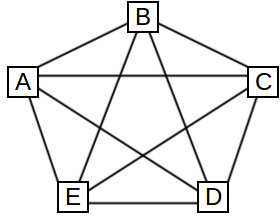
\includegraphics[scale=0.6]{rede_broadcast.jpg}
  \caption{Exemplo de $O(N^{2})$ adjac�ncias entre roteadores.}
  \label{fig:broadcast}
\end{figure}

O protocolo OSPF reduz este n�mero para somente $O(N)$ adjac�ncias ao selecionar um dos roteadores como roteador \textit{designado}. Os demais roteadores estabelecem adjac�ncias somente com o roteador designado. A Figura \ref{fig:adjacencias} mostra um rede com cinco roteadores na qual o roteador ``A'' � selecionado como roteador designado e deve manter adjac�ncia com os outros roteadores. Al�m disso, um roteador reserva � selecionado juntamente com o roteador designado. Caso o roteador designado falhe, o roteador reserva � utilizado para substitui-lo. Portanto os roteadores tamb�m devem estabelecer adjac�ncia com o roteador reserva. Neste caso, cada roteador estabelece no m�ximo tr�s adjac�ncias, uma com o roteador designado, uma com o roteador reserva e uma com os \textit{hosts} da rede; com excess�o dos roteadores designado e reserva que devem estabelecer adjac�ncias com todos os roteadores da rede.

\vspace{5 mm}

\begin{figure}[hb]
  \centering
  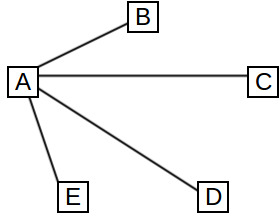
\includegraphics[scale=0.5]{adjacencias_broadcast.jpg}
  %\caption{Exemplo de $O(N)$ adjac�ncias entre o roteador designado A e os demais roteadores.}
  \caption{Exemplo de $O(N)$ adjac�ncias entre os roteadores, A � o roteador designado.}
  \label{fig:adjacencias}
\end{figure}

O procedimento de utilizar um roteador designado reduz a quantidade de tr�fego utilizado pelas mensagens de controle do protocolo \cite{Reference6}. Al�m disso, diminui o tamanho da representa��o da topologia que guarda os estados dos enlaces da rede.

O protocolo OSPF aplica o mesmo gerenciamento para redes \textit{broadcast} e redes n�o \textit{broadcast}. Os roteadores selecionam um roteador designado e um roteador reserva. As informa��es de roteamento s�o trocadas apenas com estes dois roteadores. O uso de um roteador designado n�o altera o roteamento das demais informa��es. Caminhos virtuais s�o estabelecidos  entre qualquer par de roteadores. Os pacotes s�o transmitidos diretamente sobre estes caminhos virtuais. Mas estes caminhos s�o estabelecidos apenas sob demanda. Os �nicos caminhos que ser�o usados permanentemente pelas atualiza��es de roteamento s�o os que ligam os roteadores com o roteador designado e o roteador reserva.

O protocolo OSPF permite que diversas redes adjacentes sejam agrupadas. Cada grupo, em conjunto com os enlaces entre os roteadores pertencentes ao grupo, � chamado de \textit{�rea}. Cada �rea executa uma c�pia separada do protocolo de roteamento. Isto significa que cada �rea tem sua pr�pria representa��o local da topologia, descrita por um grafo. A topologia de uma �rea � invis�vel para as demais �reas. Este isolamento permite reduzir o tr�fego das mensagens do protocolo de roteamento. Com a introdu��o de �reas, as representa��es da topologia nos roteadores deixam de ser id�nticas. Cada roteador tem um grafo separado para cada �rea em que est� conectado. Dois roteadores pertencentes � mesma �rea t�m, para essa �rea, as representa��es da topologia id�nticas. O roteamento em um sistema aut�nomo ocorre em dois n�veis, dependendo da origem e o destino de um pacote pertencerem a diferentes �reas ou � mesma �rea. No roteamento dentro de uma �rea, o pacote � encaminhado utilizando apenas informa��es obtidas dentro da �rea. Isso impede que os roteadores de uma determinada �rea influenciem de maneira nociva o roteamento das demais �reas \cite{Reference3}.

\subsection{Algoritmo de Dijkstra}

Como foi visto anteriormente, o protocolo OSPF utiliza um grafo para representar a topologia da rede. A partir deste grafo � poss�vel calcular o caminho m�nimo de uma origem para cada destino. Para encontrar estes caminhos o OSPF usa o algoritmo de Dijkstra \cite{Reference16} tamb�m chamado de algoritmo do caminho m�nimo, descrito a seguir. 

O algoritmo de Dijkstra resolve o problema de encontrar os caminhos m�nimos, a partir uma �nica origem, em um grafo direcionado $G = (V, E)$, com a fun��o peso $w : E \rightarrow R$ que mapeia as arestas para valores de pesos. O peso do caminho $p = v_0, v_1, ..., v_k$ � dado pela soma dos pesos das arestas que constituem o caminho $p$:

\vspace{5 mm}
$
w(p) = \displaystyle \sum_{i=1}^{k} w(v_{i-1}, v_i)
$
\vspace{5 mm}

O peso do caminho m�nimo de $u$ para $v$ � definido por

\vspace{5 mm}
$
\delta(u,v) = \left\{\begin{array}{ll}
min\{w(p) : u \stackrel{p}{\leadsto} v\} & se\ existe\ um\ caminho\ de\ u\ para\ v,\\
\infty & caso\ contr\acute{a}rio.
\end{array}\right.
$
\vspace{5 mm}

Um caminho m�nimo do v�rtice $u$ ao v�rtice $v$ � ent�o definido como qualquer caminho $p$ com peso $w(p) = \delta(u,v)$.

Os pesos das arestas s�o muitas vezes utilizados para representar tempo, custo, perda, ou qualquer outra quantidade que se acumula linearmente ao longo de um caminho e que se pretende minimizar. Entretanto as arestas n�o devem possuir valores negativos.

O algoritmo de Dijkstra utiliza uma t�cnica chamada relaxamento. Para cada v�rtice $v \in V$, existe um atributo $d[v]$, que � um limite superior sobre o peso de um caminho m�nimo da origem $s$ para $v$. O atributo $d[v]$ � considerado uma estimativa do caminho m�nimo. O atributo $\pi[v]$ � considerado o v�rtice antecessor ao v�rtice $v$. A Figura \ref{fig:inicializa} mostra a inicializa��o da estimativa do caimnho mais curto e seus antecessores.

\begin{figure}[hb]
\begin{algorithm}{INICIALIZA}[G, s]{}
\qfor $v\acute{e}rtice\ v \in V[G]$ \\
\qdo $d[v] \qlet \infty$ \\
$\pi[v] \qlet NIL$ \qrof\\
$d[s] \qlet 0$
\end{algorithm}
  \caption{Pseudo-c�digo do algoritmo respons�vel por inicializar os atributos $d$ e $\pi$.}
  \label{fig:inicializa}
\end{figure}


%\begin{figure}[hb]
%\begin{lstlisting}[mathescape]
%INICIALIZA(G, s)
%1:   para cada v�rtice v $\in$ V[G]
%2:      fa�a d[v] $\leftarrow$ $\infty$
%3:	    $\pi$[v] $\leftarrow$ NIL
%4:   d[s] $\leftarrow$ 0
%\end{lstlisting}
%  \caption{Pseudo-c�digo do algoritmo respons�vel por inicializar os atributos $d$ e $\pi$.}
%  \label{fig:inicializa}
%\end{figure}

Ap�s a inicializa��o, $\pi$[v] = NIL para todo $v \in V$, $d[s] = 0$ e $d[v] = \infty$ para todo $v \in V - \{s\}$. A Figura \ref{fig:relaxamento} mostra que o processo de relaxamento de uma aresta $(u, v)$ consiste em testar se � poss�vel melhorar o caminho m�nimo para $v$ encontrado at� agora, passando por $u$ e, nesse caso, atualizar $d[v]$ e $\pi[v]$. Um passo do relaxamento pode diminuir o valor da estimativa do caminho m�nimo $d[v]$ e atualizar o atributo do seu antecessor $\pi[v]$. No algoritmo de Dijkstra cada aresta � relaxada exatamente uma vez. O c�digo a seguir executa um passo do relaxamento � aresta $(u, v)$.

\begin{figure}[hb]
\begin{algorithm}{RELAXAMENTO}[u, v, w]{}
\qif $d[v] > d[u] + w(u, v)$ \\
\qthen $d[v] \qlet d[u] + w(u, v)$ \\
$\pi[v] \qlet u$ \qfi\\
\end{algorithm}
  \caption{Pseudo-c�digo do algoritmo respons�vel pelo relaxamento da aresta $(u, v)$.}
  \label{fig:relaxamento}
\end{figure}

%\begin{figure}[hb]
%\begin{lstlisting}[mathescape]
%RELAXAMENTO(u, v, w)
%1:   se d[v] > d[u] + w(u, v)
%2:      ent�o d[v] $\leftarrow$ d[u] + w(u, v)
%3:            $\pi$[v] $\leftarrow$ u
%\end{lstlisting}
%  \caption{Pseudo-c�digo do algoritmo respons�vel pelo relaxamento da aresta $(u, v)$.}
%  \label{fig:relaxamento}
%\end{figure}
 
A Figura \ref{fig:execucao} mostra que algoritmo de Dijkstra mant�m um conjunto de v�rtices $S$, no qual o peso de alguns dos caminhos m�nimos $s$ j� foram determinados. O algoritmo seleciona repetidamente o v�rtice $u \in V - S$ com a menor estimativa do caminho m�nimo, acrescenta $u$ a $S$, e aplica o relaxamento em todas as arestas que tem origem em $u$. � utilizada uma fila de v�rtices $Q$ com prioridade baseada em seus valores da estimativa do caminho m�nimo $d$.

\begin{figure}[hb]
\begin{algorithm}{DIJKSTRA}[G, w, s]{}
$INICIALIZA(G, s)$ \\
$S \qlet \emptyset$ \\
$Q \qlet V[G]$ \\
\qwhile $Q \neq \emptyset$ \\
\qdo $u \qlet EXTRAI-MINIMO(Q)$ \\
$S \qlet S \cup {u}$ \\
\qfor $v\acute{e}rtice\ v \in Adj[u]$ \\
\qexec $RELAXAMENTO(u, v, w)$ \qrof\qend\\
\end{algorithm}
  \caption{Pseudo-c�digo do algoritmo de Dijkstra.}
  \label{fig:dijkstra}
\end{figure}

%\begin{figure}[hb]
%\begin{lstlisting}[mathescape]
%DIJKSTRA(G, w, s)
%1:   INICIALIZA(G, s)
%2:   S $\leftarrow$ $\emptyset$
%3:   Q $\leftarrow$ V[G]
%4:   enquanto Q $\neq$ $\emptyset$
%5:      fa�a u $\leftarrow$ EXTRAI-MINIMO(Q)
%6:           S $\leftarrow$ S $\cup$ {u}
%7:           para cada v�rtice v $\in$ Adj[u]
%8:              execute RELAXAMENTO(u, v, w)
%\end{lstlisting}
%  \caption{Pseudo-c�digo do algoritmo de Dijkstra.}
%  \label{fig:dijkstra}
%\end{figure}

A primeira linha do algoritmo executa a inicializa��o dos valores de $d$ e $\pi$ e a segunda linha inicializa o conjunto $S$ como vazio. A terceira linha inicializa a fila de prioridade $Q$ para conter todos os v�rtices em $V$, uma vez que $S = \emptyset$. O algoritmo mant�m a invariante que $Q = V - S$ no in�cio de cada itera��o do la�o das linhas 4 at� 8. Em cada itera��o deste la�o, um v�rtice $u$ � extra�do de $Q = V - S$ e adicionado ao conjunto $S$, mantendo assim o invariante. Na primeira itera��o, $u = s$. Portanto, o v�rtice $u$ tem a menor estimativa do caminho m�nimo de qualquer v�rtice em $V - S$. Em seguida, nas linhas 7 e 8 acontece o relaxamento de cada aresta $(u, v)$ com origem em $u$. No relaxamento, a estimativa $d[v]$ e do antecessor $\pi[v]$ s�o atualizados se o caminho m�nimo para $v$ pode ser melhorado, passando por $u$. � poss�vel observar que os v�rtices nunca s�o inseridos em $Q$ ap�s a terceira linha e que cada v�rtice � extra�do de $Q$ e adicionado em $S$ exatamente uma vez, de modo que o la�o das linhas 4 a 8 itera exatamente $|V|$ vezes.

%A Figura \ref{fig:execucao} mostra uma execu��o do algoritmo de Dijkstra, na qual a origem $s$ � o v�rtice mais � esquerda. As estimativas de caminho m�nimo s�o mostradas dentro dos v�rtices e as arestas sombreadas indicam os valores do antecessor. V�rtices pretos est�o no conjunto $S$, e v�rtices brancos est�o na da fila $Q = V - S$. (a) Situa��o, pouco antes da primeira itera��o do la�o das linhas 4 a 8. O v�rtice sombreado tem o valor $d$ m�nimo e � escolhido como v�rtice $u$ na linha 5. (b) - (f) mostram as situa��es depois de cada itera��o sucessiva do la�o. O v�rtice sombreado em cada parte � escolhido como v�rtice $u$ na linha 5 da pr�xima itera��o. Os valores de $d$ e $\pi$ mostrados na parte (f) s�o os valores finais.

A Figura \ref{fig:execucao} mostra uma execu��o do algoritmo de Dijkstra, na qual a origem � o v�rtice $s$, mais � esquerda. Os valores das estimativas de caminho m�nimo s�o mostrados dentro dos v�rtices. Os v�rtices pretos est�o no conjunto $S$, e os v�rtices brancos est�o na fila de prioridade $Q = V - S$. O v�rtice sombreado de cada estado ser� selecionado na fila de prioridade $Q$, pois tem o menor valor da estimativa do caminho m�nimo. O estado incial (a) mostra o grafo ap�s a inicializa��o. No estado (b), o v�rtice $s$ � selecionado e removido da fila $Q$. Em seguida, � aplicado o relaxamento nas arestas com origem em $s$ e as estimativas de caminho m�nimo dos v�rtices $t$ e $y$ recebem novos valores. No estado (c), o v�rtice $y$ � selecionado na fila $Q$. Em seguida, � aplicado o relaxamento. Este processo se repete at� que a fila $Q$ fique vazia. O estado (f) mostra os valores finais das estimativas de caminho m�nimo e as arestas sombreadas indicam os v�rtices antecessores.

\begin{figure}[hb]
  \centering
  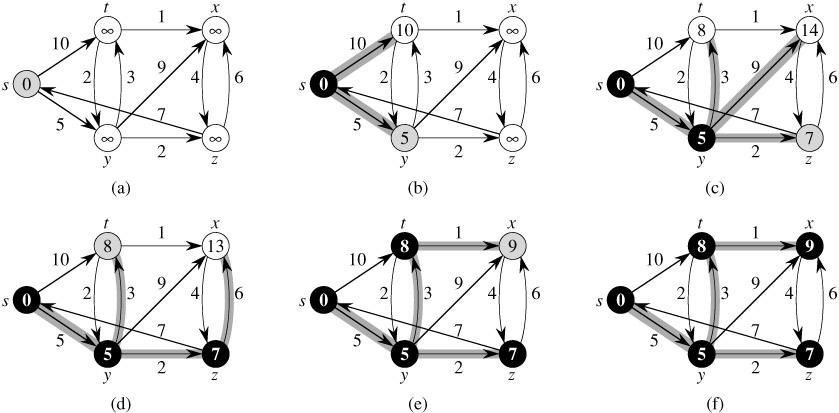
\includegraphics[scale=1]{fig24_6.jpg}
  \caption{Um exemplo de execu��o do algoritmo de Dijkstra \cite{Reference16}.}
  \label{fig:execucao}
\end{figure}

%Dijkstra's algorithm [75] appeared in 1959, but it contained no mention of a priority queue.

%Dijkstra propos um algoritmo que ele chamou de \textit{Shortest Path First (SPF)}. O algoritmo \textit{SPF} calcula o caminho mais curto entre um roteador de origem e os outros roteadores na rede. Ele separa os roteadores em dois conjuntos: o conjunto de roteadores avaliados, E, para os quais s�o conhecidos os caminhos mais curtos, e o conjunto de roteadores restantes, R. O algoritmo tamb�m mant�m uma lista ordenada de caminhos, O. O algoritmo funciona da seguinte maneira. Primeiro, � preciso inicializar o conjunto E com apenas o roteador de origem S e o conjunto R contendo todos os outros roteadores. Al�m disso, inicializar a lista de caminhos O para conter os enlaces que possuem origem no roteador S. Cada um desses caminhos tem um custo igual a m�trica do enlace correspondente. Para finalizar a etapa inicial do algoritmo, � necess�rio ordenar a lista O por m�tricas crescentes. Na segunda etapa, se a lista O est� vazia, ou se o primeiro caminho em O tem uma custo de infinito, ent�o marcar todos os roteadores restantes em R como inacess�veis. Caso isso aconte�a o algoritmo encerra. Caso contr�rio remover o caminho mais curto P da lista O. Sendo V o �ltimo roteador em P, se V j� est� no conjunto E, ent�o voltar para a segunda etapa. Caso contr�rio, mover o roteador V do conjunto R para o conjunto E. Em seguida, construir um conjunto de novos caminhos candidatos pela concatena��o do caminho P e cada um dos enlaces com origem em V. O custo desses caminhos � a soma de P e da m�trica do enlace anexado a P. Al�m disso, inserir os novos caminhos na lista ordenada O e voltar para a segunda etapa.

\subsection{Os Protocolos Internos ao OSPF}

O protocolo OSPF � composto de tr�s subprotocolos: \textit{Hello}, \textit{Exchange} e \textit{Flooding} \cite{Reference3}, s�o descritos a seguir. A descri��o � baseada em \cite{Reference1,Reference3}.

\subsubsection{O Protocolo Hello}

%O protocolo \textit{Hello} � respons�vel por estabelecer e manter rela��es de vizinhan�a. Ele tamb�m garante que a comunica��o entre vizinhos seja bidirecional. Os pacotes \textit{Hello} s�o transmitidos periodicamente em todas as interfaces do roteador. Em redes \textit{broadcast}, o protocolo \textit{Hello} tamb�m tem a fun��o de eleger um roteador designado para a rede. O protocolo \textit{Hello} funciona de forma diferente em redes \textit{broadcast} e redes ponto-a-ponto. Em redes \textit{broadcast}, cada roteador envia pacotes \textit{Hello} periodicamente aos demais roteadores. Isto permite que vizinhos sejam descobertos de maneira din�mica. Os pacotes \textit{Hello} cont�m a lista de roteadores que enviaram pacotes \textit{Hello} recentemente. Em redes ponto-a-ponto redes, um roteador envia pacotes \textit{Hello} para todos os vizinhos com os quais podem se comunicar diretamente. Estes vizinhos podem ser descobertos dinamicamente atrav�s de um protocolo, tal como \textit{ARP} Reverso \cite{Reference11}.

O protocolo \textit{Hello} � utilizado para dois prop�sitos. Verificar o estado dos enlaces e eleger um roteador designado e um roteador reserva. Para isso, pacotes denominados \textit{hello} s�o enviados pelos roteadores a cada \textit{hello-interval} segundos. Os pacotes incluem o endere�o do roteador designado, ou 0 se ainda n�o houver roteador designado, e o endere�o do roteador reserva ou 0. Al�m disso, tamb�m incluem uma lista de todos os vizinhos dos quais um pacote \textit{hello} foi recebido nos �ltimos \textit{dead-interval} segundos. Ambos os intervalos \textit{hello-interval} e \textit{dead-interval} s�o par�metros dos enlaces que s�o configurados pelo administrador da rede. A liga��o entre dois roteadores � dita \textit{operacional} se os pacotes podem fluir em ambas as dire��es. A conectividade bidirecional � identificada pela lista de roteadores conhecidos por um roteador vizinho. Se o identificador do roteador local n�o estiver listado nos pacotes \textit{hello} enviados pelos roteadores vizinhos, isso significa que eles ainda n�o receberam os pacotes \textit{hello} enviados pelo roteador local. O enlace � ent�o declarado de \textit{sentido �nico} e n�o pode ser usado para o roteamento. Se o roteador local est� listado nos pacotes \textit{hello} dos roteadores vizinhos, ent�o o enlace � \textit{bidirecional}. 

Depois de estabelecer uma conex�o bidirecional, os roteadores come�am a determinar suas adjac�ncias. Primeiro � preciso selecionar o roteador designado e o roteador reserva. O processo de elei��o usa o campo de \textit{prioridade} presente nos pacotes \textit{hello}. Cada roteador � configurado com uma prioridade, que varia entre 0 e 255. Como resultado da elei��o � selecionado o roteador com a maior prioridade. Se o roteador de maior prioridade fica inativo, outro ser� selecionado; esta sele��o permanecer� mesmo depois do roteador de maior prioridade se tornar ativo novamente. Roteadores com prioridade zero, nunca s�o selecionados como roteador designado.

Imediatamente ap�s os enlaces se tornarem ativos, o roteador permanece em um estado de \textit{espera} durante um intervalo igual ao \textit{dead-interval}. Durante este intervalo, o roteador ir� transmitir pacotes de \textit{hello}, mas n�o vai se candidatar a roteador designado ou reserva. Ele ir� receber pacotes \textit{hello} e inicializar os identificadores dos roteadores designado e reserva da seguinte forma. Para cada vizinho, o roteador guarda a prioridade do vizinho e o estado do enlace. Al�m disso, ele guarda se o vizinho se candidata como roteador designado ou reserva. Se um ou v�rios vizinhos se candidatam como roteador reserva, aquele com maior prioridade � selecionado. Em caso de empate, o roteador com o maior identificador � selecionado. Se nenhum vizinho se candidata a roteador reserva, o vizinho com a maior prioridade � selecionado ou, em caso de empate, aquele com o maior ID. Se um ou v�rios vizinhos se candidatam a roteador designado, aquele com a maior prioridade � selecionado como roteador designado. Em caso de empate, o roteador com o maior identificador � selecionado. Se nenhum vizinho se candidata a roteador designado, o reserva � \textit{promovido}. Um roteador n�o pode se candidatar a ambos roteador designado e reserva. Assim, se for preciso promover o roteador reserva para roteador designado, tamb�m ser� necess�rio eleger um novo roteador reserva.

\subsubsection{O Protocolo Exchange}

Quando dois roteadores estabelecem conectividade bidirecional, eles devem sincronizar sua representa��o local da topologia da rede. Em redes \textit{broadcast}, isso ocorre entre os roteadores e o roteador designado ou o roteador reserva. A sincroniza��o inicial � realizada atrav�s do protocolo \textit{Exchange}. O protocolo \textit{Flooding}, em seguida, � respons�vel por manter as representa��es da topologia da rede sincronizadas. O protocolo \textit{Exchange} � assim�trico. A primeira etapa do protocolo tem a fun��o de selecionar um mestre e um escravo. Depois de concordar sobre esses pap�is, os dois roteadores trocam a descri��o de seus grafos, que representam a topologia da rede. Cada um ir� listar os enlaces que ser�o requisitados em seguida. 

No pacote utilizado pelo protocolo \textit{Exchange} existem tr�s \textit{bits} utilizados para controle: I (Inicializa), M (Mais) e MS (Mestre-Escravo). O roteador que pretende iniciar o procedimento de sincroniza��o envia um pacote vazio, com os \textit{bits} I, M e MS definidos como 1 e o contador definido para um valor arbitr�rio, n�o visto anteriormente pelo outro roteador. O outro roteador concorda em fazer a fun��o de \textit{escravo} durante a sincroniza��o enviando um pacote igual ao que foi recebido, por�m com o \textit{bit} MS definido como 0. Uma vez que os pap�is foram distribu�dos, o mestre ir� enviar a descri��o dos enlaces presentes na representa��o local da topologia em uma sequ�ncia de pacotes, nos quais o \textit{bit} I ser� definido como 0, o \textit{bit} MS definido como 1 e o \textit{bit} M definido como 1, exceto para o �ltimo pacote. Os pacotes t�m sequ�ncia numerada e devem ser enviados um de cada vez. Depois de cada pacote ser enviado, o escravo ir� enviar uma confirma��o de que recebeu o pacote. Os pacotes de confirma��o cont�m a descri��o dos enlaces presentes na representa��o local da topologia do roteador escravo. Se a confirma��o n�o for recebida dentro do intervalo de retransmiss�o, o mestre retransmite o seu pacote. Quando o escravo recebe um pacote com o valor do contador igual ao valor do pacote anterior, deve retransmitir o �ltimo pacote de confirma��o. Quando o mestre transmite sua �ltima descri��o dos enlaces, ele vai definir o \textit{bit} M como 0. Se o escravo ainda tem descri��es de enlaces para transmitir, ele ir� enviar uma confirma��o com o \textit{bit} M definido como 1. O mestre continuar� enviando pacotes de descri��o vazios com o \textit{bit} M definido como 0. Como consequ�ncia, continuar� aceitando confirma��es, at� que eventualmente receba uma confirma��o com o \textit{bit} M definido como 0. Nesse ponto a primeira etapa da sincroniza��o est� completa.

Durante a sincroniza��o, o mestre e o escravo processam as descri��es dos estados de enlace que se encontram nos pacotes e nas confirma��es. Primeiro verificam se n�o h� um enlace com a mesma descri��o na represent��o local da topologia. Al�m disso verificam, atrav�s do valor de um contador, se esse enlace n�o est� desatualizado. Se alguma das condi��es for satisfeita, os roteadores devem colocar a descri��o do enlace em uma lista de \textit{enlaces pendentes}. Na segunda etapa da sincroniza��o, os roteadores ir�o solicitar informa��es dos enlaces pendentes. Ap�s receber uma solicita��o, cada roteador deve enviar um ou mais pacotes contendo um conjunto de atualiza��es de estado de enlace. A transmis�o destes pacotes utiliza exatamente os mesmos procedimentos do protocolo \textit{Flooding} descrito a seguir.

% indicado o uso do horario do dia como valor arbitr�rio.
%De fato, v�rios eventos podem perturbar essa troca, por exemplo, a perda de pacotes ou uma \textit{colis�o} se ambos os roteadores tentar inicializar o processo simultaneamente. A prote��o contra perdas de pacotes � atrav�s de tempos de espera: na aus�ncia de confirma��o, o pacote inicial � repetido a cada segundo \textit{retransmitir-interval}. a resolu��o de colis�o � atrav�s de um algoritmo simples de desempate: se um roteador est� � espera de um reconhecimento e recebe um pedido que vai comparar o endere�o de envio para o seu pr�prio. Se o endere�o de envio � maior do que a sua pr�pria, ele ir� aceitar a rola escravo e confirmar o pacote, caso contr�rio, ele ir� simplesmente ignorar o pacote de entrada, como o seu pr�prio pacote ser� reconhecido mais tarde pelo roteador remoto.

\subsubsection{O Protocolo Flooding}

%Quando um enlace muda de estado, o roteador respons�vel por esse enlace vai transmitir o novo estado do enlace. O protocolo \textit{Flooding} � usado para transmitir as atualiza��es do roteamento, mas tamb�m � usado para sincronizar a idade dos registros nos bancos de dados.

Quando um enlace muda de estado, o roteador respons�vel por esse enlace vai transmitir uma mensagem com a nova vers�o do estado do enlace. Para cada enlace, existe um contador que � comparado com o valor na representa��o local da topologia. Se o valor do contador indicar que o enlace presente na mensagem recebida � novo, ent�o a mensagem recebida deve ser retransmitida em todas as interfaces. Em qualquer caso, o roteador que enviou a mensagem deve aguardar uma confirma��o de recebimento. Para tornar o protocolo \textit{Flooding} confi�vel, o roteador deve retransmitir suas atualiza��es em intervalos regulares at� que receba a confirma��o. Cada pacote de confirma��o pode ser respons�vel por informar o recebimento de uma ou mais mensagens, com informa��es de estado de enlace. Portanto � normal atrasar a sua transmiss�o, a fim de agrupar a confirma��o, de recebimento do estado de v�rios enlaces, em um �nico pacote. Este atraso deve ser curto, a fim de evitar retransmi��es desnecess�rias. 


\chapter{Instalando o Simulador NS-3 Para Executar OSPF}
\label{Instalando o Simulador NS-3 Para Executar OSPF}

Este cap�tulo descreve os procedimentos necess�rios para instalar e configurar o simulador de redes \textit{Network Simulator 3} (NS-3) \cite{Reference12}. Inicialmente, s�o apresentadas as caracter�sticas e as funcionalidades do NS-3. Em seguida, s�o descritas as instru��es utilizadas para instalar e configurar o NS-3.
% Primeiro, s�o apresentadas as caracter�sticas e as funcionalidades do \textit{NS-3}. Em seguida, s�o descritos os procedimentos necess�rios para o uso do \textit{NS-3}.% O cap�tulo termina com uma descri��o detalhada do protocolo OSPF.

\lstset{
  backgroundcolor=\color{mybckg},  % choose the background color; you must add \usepackage{color} or \usepackage{xcolor}
  basicstyle=\footnotesize,       % the size of the fonts that are used for the code
  breakatwhitespace=false,         % sets if automatic breaks should only happen at whitespace
  breaklines=true,                 % sets automatic line breaking
  %captionpos=b,                    % sets the caption-position to bottom
  %commentstyle=\color{mygreen},    % comment style
  deletekeywords={...},            % if you want to delete keywords from the given language
  escapeinside={\%*}{*)},          % if you want to add LaTeX within your code
  extendedchars=true,              % lets you use non-ASCII characters; for 8-bits encodings only, does not work with UTF-8
  frame=single,                    % adds a frame around the code
  keepspaces=true,                 % keeps spaces in text, useful for keeping indentation of code (possibly needs columns=flexible)
  columns=flexible,
  %keywordstyle=\color{blue},       % keyword style
  %language=bash,                   % the language of the code
  %morekeywords={*,...},            % if you want to add more keywords to the set
  %numbers=left,                    % where to put the line-numbers; possible values are (none, left, right)
  %numbersep=5pt,                   % how far the line-numbers are from the code
  %numberstyle=\tiny\color{mygray}, % the style that is used for the line-numbers
  rulecolor=\color{black},         % if not set, the frame-color may be changed on line-breaks within not-black text (e.g. comments (green here))
  %showspaces=false,                % show spaces everywhere adding particular underscores; it overrides 'showstringspaces'
  %showstringspaces=false,          % underline spaces within strings only
  %showtabs=false,                  % show tabs within strings adding particular underscores
  %stepnumber=2,                    % the step between two line-numbers. If it's 1, each line will be numbered
  %stringstyle=\color{mymauve},     % string literal style
  tabsize=2,                       % sets default tabsize to 2 spaces
  %title=\lstname                   % show the filename of files included with \lstinputlisting; also try caption instead of title
  basicstyle=\ttfamily
}

%----------------------------------------------------------------------------------------
%	SECTION 1
%----------------------------------------------------------------------------------------
\section{Caracter�sticas e Funcionalidades}

%ns-2 build of 2009 is not actively maintainer (and is not being accepted for journal publications)

O NS-3 � um simulador de rede de eventos discretos, voltado principalmente para pesquisa e uso educacional \cite{Reference12}. O simulador NS-3 � um software livre, licenciado sob a licen�a GNU GPLv2, e est� dispon�vel publicamente para a pesquisa e desenvolvimento.

O simulador NS-3 oferece suporte � pesquisa em redes IP e redes n�o baseadas em IP. No entanto, a grande maioria de seus usu�rios se concentra em simula��es de redes sem fio que envolvem modelos para, por exemplo, Wi-Fi, WiMAX ou LTE. 

Outra funcionalidade do simulador est� na reutiliza��o de aplica��es reais. Atualmente, est�o sendo testados m�dulos do NS-3 para a execu��o de aplica��es reais e o uso dos protocolos da Internet implementados no kernel do Linux.

O NS-3 � constru�do como um sistema de bibliotecas de \textit{software}. Estas bibliotecas s�o escritas na linguagem orientada a objetos conhecida como C++. Entretanto os \textit{scripts} de simula��o n�o precisam ser escritos em C++, eles podem ser escritos em Pyhton.

%----------------------------------------------------------------------------------------
%	SECTION 2
%----------------------------------------------------------------------------------------
\section{Instala��o e Configura��o}

Atualmente, existe uma ferramenta para auxiliar na instala��o do simulador NS-3 chamada \textit{Bake} \cite{Reference17}. \textit{Bake} � uma ferramenta utilizada na instala��o e configura��o do NS-3 e seus m�dulos. A m�quina utilizada para simula��es do protocolo OSPF usa um sistema operacional baseado no Ubuntu 12.04. Portanto, os pacotes necess�rios foram instalados atrav�s do gerenciador de pacotes do Ubuntu, o \textit{apt-get}. A seguir � apresentada uma s�rie de procedimentos necess�rios para o uso do simulador NS-3.

Para usar a ferramenta \textit{Bake} � preciso ter a linguagem Python (vers�o 2.6 ou superior) instalada. Al�m disso � necess�ria a ferramenta de controle de vers�o Mercurial utilizada para fazer o \textit{download} do \textit{Bake}.

\begin{lstlisting}
sudo apt-get install python python-dev mercurial
\end{lstlisting}

Em seguida � necess�rio fazer o \textit{download} da ferramenta \textit{Bake} usando o Mercurial.

\begin{lstlisting}
hg clone http://code.nsnam.org/bake
\end{lstlisting}

Isso cria um reposit�rio da ferramenta \textit{Bake} no diret�rio. Para facilitar o uso da ferramenta \textit{Bake}, � preciso adicionar ao \textit{PATH} o endere�o do diret�rio onde foi criado o reposit�rio do \textit{Bake}.

\begin{lstlisting}
export BAKE_HOME=`pwd`/bake
export PATH=$PATH:$BAKE_HOME
export PYTHONPATH=$PYTHONPATH:$BAKE_HOME
\end{lstlisting}

Depois disso, � poss�vel utilizar o \textit{Bake} para encontrar os pacotes pendentes. Para descobrir quais pacotes estam faltando e s�o necess�rios para a instala��o do NS-3 e seus m�dulos basta executar o segtuinte comando:

\begin{lstlisting}
bake.py check
\end{lstlisting}

Com isso � poss�vel visualizar a seguinte lista de pacotes a serem utilizados:

Compilador GNU C++.

\begin{lstlisting}
sudo apt-get install gcc g++
\end{lstlisting}

CVS, GIT e Bazaar.

\begin{lstlisting}
sudo apt-get install cvs git-core bzr
\end{lstlisting}

Ferramentas Tar, Unzip e Unrar. Al�m dos compressores de dados 7z e XZ.

\begin{lstlisting}
sudo apt-get install tar unzip unrar p7zip-full xz-utils
\end{lstlisting}

Make e cMake.

\begin{lstlisting}
sudo apt-get install make cmake
\end{lstlisting}

Patch tool.

\begin{lstlisting}
sudo apt-get install patch
\end{lstlisting}

Autoreconf tool.

\begin{lstlisting}
sudo apt-get install autoconf
\end{lstlisting}

Tamb�m foram instalados alguns pacotes adicionais para visualizar os resultados das simula��es e fazer depura��o de c�digo.

\begin{lstlisting}
sudo apt-get install tcpdump gdb valgrind
\end{lstlisting}

Na implementa��o do NS-3 existe um conjunto de classes que tem o objetivo de simular o funcionamento de um protocolo de roteamento baseado no OSPF. Como foi visto anteriormente, o protocolo OSPF � dividido em tr�s subprotocolos: os protocolos \textit{Hello}, \textit{Exchange} e \textit{Flooding}. Entretanto, a implementa��o do simulador NS-3 n�o simula o funcionamento dos protocolos \textit{Hello} e \textit{Flooding}. � poss�vel observar que somente o funcionamento do protocolo \textit{Exchange} � simulado no NS-3. Sendo assim, o NS-3 n�o simula o funcionamento completo do protocolo OSPF. Deste modo, o estudo do protocolo OSPF fica muito limitado. Para aprofundar a an�lise do OSPF � necess�rio o uso de uma ferramenta adicional. Existe um m�dulo para o simulador NS-3 chamado \textit{Direct Code Execution} (DCE) \cite{Reference13}. O m�dulo DCE permite a execu��o de algumas aplica��es reais dentro do NS-3. Umas das aplica��es que o DCE fornece suporte � a implementa��o do protocolo OSPF presente na \textit{Quagga Routing Suite} \cite{Reference14}. Ao utilizar o m�dulo DCE � poss�vel ampliar o estudo do protocolo OSPF e deix�-lo mais abragente. O DCE precisa dos seguintes pacotes.

\begin{lstlisting}
sudo apt-get install automake flex bison wget indent pkg-config gawk libssl-dev libsysfs-dev libc6-dbg
\end{lstlisting}

Neste ponto todos os pacotes necess�rios para instalar o NS-3 e simular o OSPF est�o instalados. Agora � preciso configurar o \textit{Bake} para utilizar os seguintes m�dulos. O m�dulo dce-quagga que permite usar o protocolo OSPF, implementado pelo Quagga, nas simula��es. Al�m do m�dulo dce-linux que permite utilizar a implementa��o do protocolo IP nativo do Linux.

\begin{lstlisting}
mkdir dce
cd dce
bake.py configure -e dce-linux-1.1 -e dce-quagga-1.1
\end{lstlisting}

� poss�vel vizualizar quais m�dulos ser�o utilizados e os requisitos espec�ficos do sistema para esta configura��o, atrav�s do seguinte comando.

\begin{lstlisting}
bake.py show
\end{lstlisting}

Por �ltimo, para baixar, configurar e instalar o simulador NS-3 al�m dos m�dulos necess�rios basta executar o segtuinte comando:

\begin{lstlisting}
bake.py deploy
\end{lstlisting}

Ap�s a execu��o do comando anterior � poss�vel verificar se a instala��o do m�dulo Quagga foi bum sucedida.

\begin{lstlisting}
cd source/ns-3-dce
./test.py -s dce-quagga
\end{lstlisting}

Depois da conclus�o da instala��o, o simulador NS-3 est� dispon�vel. Al�m disso, o protocolo OSPF, implementado na \textit{Quagga Routing Suite}, est� acess�vel para realizar simula��es atrav�s do NS-3.



\chapter{Simula\c{c}\~ao do OSPF no NS-3}
\label{Simulacao do OSPF no NS-3}

Este cap�tulo, descreve a execu��o de simula��es com o protocolo OSPF no simulador de redes NS-3. Primeiro, s�o apresentadas as instru��es utilizadas para criar a simula��o no NS-3. Em seguida, s�o descritos os procedimentos necess�rios para utilizar o m�dulo DCE nas simula��es do OSPF. O cap�tulo termina com os resultados das simula��es que utilizam o m�dulo DCE.

%simula��es que utilizam os recursos dispon�veis no simulador NS-3

%----------------------------------------------------------------------------------------
%	SECTION 1
%----------------------------------------------------------------------------------------
\section{OSPF no NS-3}

A primeira etapa para realizar a simula��o de uma rede � definir a topologia desta rede. A Figura \ref{fig:topologia} mostra a topologia escolhida para as simula��es, com cinco roteadores contectados por enlaces pono-a-ponto.

\begin{figure}[hb]
  \centering
  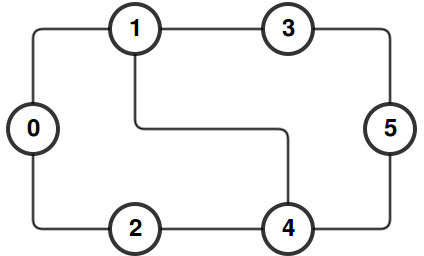
\includegraphics[scale=0.5]{rede_tg.jpg}
  \caption{Representa��o da topologia da rede utilizada nas simula��es do protocolo OSPF.}
  \label{fig:topologia}
\end{figure}

%Em seguida, � necess�rio montar a topologia da rede no NS-3. Este procedimento � dividido em diversas etapas, descritas a seguir.

Em seguida, � necess�rio montar a topologia da rede no NS-3. Por�m, antes de escrever c�digos no NS-3 � importante entender os conceitos e abstra��es do sistema.

Na Internet, um dispositivo computacional que conecta-se a uma rede � chamado de \textit{host}. Devido ao fato do NS-3 ser um simulador de rede, e n�o um simulador da Internet, o termo \textit{host} � intencionalmente n�o utilizado, pois est� intimamente associado com a Internet e seus protocolos. Ao inv�s disso, � utilizado o termo \textit{node} (n�) que � um termo mais gen�rico e tamb�m usado por outros simuladores. A abstra��o de um dispositivo computacional b�sico � chamado ent�o de n�. Essa abstra��o � representada em C++ pela classe \textit{Node}. Esta classe fornece m�todos para gerenciar as representa��es de dispositivos computacionais nas simula��es. O n� deve ser pensado como um computador no qual se adicionam funcionalidades, tal como aplicativos, pilhas de protocolos e perif�ricos com seus \textit{drivers} associados que permitem ao computador executar tarefas �teis.

Normalmente, programas de computador s�o divididos em duas classes. \textit{Programas de sistema} que organizam recursos do computador, tais como mem�ria, processador, disco, rede, entre outros. Tais programas normalmente n�o s�o utilizados diretamente pelos usu�rios. Na maioria das vezes, os usu�rios fazem uso de \textit{aplica��es}, que usam os recursos controlados pelos programas de sistema para atingir seus objetivos. Geralmente, a separa��o entre programas de sistema e aplica��es de usu�rios � feita pela mudan�a no n�vel de privil�gios que acontece na troca de contexto feita pelo sistema operacional. No NS-3, n�o existe um conceito de sistema operacional real, n�o h� o conceito de n�veis de privil�gios nem chamadas de sistema. H� apenas aplica��es que s�o executadas nos n�s para uma determinada simula��o. No NS-3, a abstra��o b�sica para um programa de usu�rio que gera alguma atividade a ser simulada � a aplica��o. Esta abstra��o � representada em C++ pela classe \textit{Application}, que fornece m�todos para gerenciar a representa��o de suas vers�es de aplica��es a serem simuladas.
% Os desenvolvedores devem especializar a classe Application para criar novas aplica��es. Neste tutorial ser�o utilizadas duas especializa��es da classe Application, chamadas UdpEchoClientApplication e UdpEchoServerApplication. Estas aplica��es comp�em um modelo cliente/servidor usado para gerar pacotes simulados de eco na rede.

No mundo real, computadores est�o conectados em uma rede. Normalmente, o meio sobre o qual os dados trafegam � chamada de canal (\textit{channel}). Quando um cabo Ethernet � ligado ao conector na parede, na verdade est� se conectando a um canal de comunica��o Ethernet. No mundo simulado do NS-3, um n� � conectado a um objeto que representa um canal de comunica��o. A abstra��o de canal de comunica��o � representada em C++ pela classe \textit{Channel}. A classe textit{Channel} fornece m�todos para gerenciar objetos de comunica��o de sub-redes e n�s conectados a eles.
% Os Channels tamb�m podem ser especializados por desenvolvedores (no sentido de programa��o orientada a objetos). Uma especializa��o de Channel pode ser algo como um simples fio. Pode tamb�m ser algo mais complexo, como um comutador Ethernet ou ainda ser uma rede sem fio (wireless) em um espa�o tridimensional com obst�culos. Neste tutorial, s�o utilizadas vers�es especializadas de Channel chamadas CsmaChannel, PointToPointChannel e WifiChannel. O CsmaChannel, por exemplo, � uma vers�o do modelo de rede que implementa controle de acesso ao meio CSMA (Carrier Sense Multiple Access). Ele fornece uma funcionalidade similar a uma rede Ethernet.

Para conectar os computadores em uma rede � necess�rio uma placa de rede. A placa de rede n�o funciona sem o driver que a controle. No Unix (ou Linux), um perif�rico (como a placa de rede) � classificado como um dispositivo (\textit{device}). As placas de rede, tamb�m chamadas de dispositivos de rede (\textit{net devices}), s�o controladas atrav�s de \textit{drivers} de dispositivo de rede (\textit{network device drivers}). No NS-3 a abstra��o do \textit{dispositivo de rede} cobre tanto o \textit{hardware} (placa de rede) quanto o \textit{software} (\textit{driver}). Um dispositivo de rede � ``instalado'' em um n� para permitir que este se comunique com outros na simula��o, usando os canais de comunica��o (\textit{channels}). Assim como em um computador real, um n� pode ser conectado a mais que um canal via m�ltiplos dispositivos de rede. A abstra��o do dispositivo de rede � representado em C++ pela classe \textit{NetDevice}, que fornece m�todos para gerenciar conex�es para objetos \textit{Node} e \textit{Channel}.
% Os dispositivos, assim como os canais e as aplica��es, tamb�m podem ser especializados. V�rias vers�es do NetDevice s�o utilizadas neste tutorial, tais como: CsmaNetDevice, PointToPointNetDevice e WifiNetDevice. Assim como uma placa de rede Ethernet � projetada para trabalhar em uma rede Ethernet, um CsmaNetDevice � projetado para trabalhar com um CsmaChannel. O PointToPointNetDevice deve trabalhar com um PointToPointChannel e o WifiNetNevice com um WifiChannel.

S�o necess�rias diversas opera��es distintas para criar um dispositivo, instalar o dispositivo em um n�, configurar a pilha de protocolos no n� em quest�o e por fim, conectar o dispositivo a um canal. Al�m disso � necess�rio conectar m�ltiplos dispositivos e ent�o fazer a interconex�o das v�rias redes. Para facilitar o trabalho, s�o disponibilizados objetos que s�o assistentes de topologia (\textit{topology helpers}), que combinam estas opera��es distintas de modo conveniente. A seguir s�o utilizados diversos destes assistentes para montar a topologia da rede utilizada nas simula��es.

As pr�ximas duas linhas de c�digo criam os objetos do tipo \textit{Node} que representar�o os roteadores na simula��o.

\begin{lstlisting}
NodeContainer routers;
routers.Create (6);
\end{lstlisting}

O assistente \textit{NodeContainer} fornece uma forma conveniente de criar, gerenciar e acessar qualquer objeto \textit{Node} que criamos para executar a simula��o. A primeira linha declara um \textit{NodeContainer} chamado \textit{routers}. A segunda linha chama o m�todo \textit{Create} sobre o objeto \textit{routers} e pede para criar seis n�s.

%Primeiro, � preciso criar objetos do tipo \textit{Node} que representar�o os roteadores na simula��o. Nas instru��es � declarado um \textit{NodeContainer} chamado de routers. Em seguida � chamado o m�todo \textit{Create} sobre o objeto routers para criar seis n�s.

%\begin{lstlisting}
%NodeContainer routers;
%routers.Create (6);
%\end{lstlisting}

%Em seguida os objetos criados s�o agrupados.

%\begin{lstlisting}
%NodeContainer ptp01 (routers.Get (0), routers.Get (1));
%NodeContainer ptp02 (routers.Get (0), routers.Get (2));
%NodeContainer ptp13 (routers.Get (1), routers.Get (3));
%NodeContainer ptp14 (routers.Get (1), routers.Get (4));
%NodeContainer ptp24 (routers.Get (2), routers.Get (4));
%NodeContainer ptp35 (routers.Get (3), routers.Get (5));
%NodeContainer ptp45 (routers.Get (4), routers.Get (5));
%\end{lstlisting}

%O assistente \textit{NodeContainer} fornece uma forma conveniente de criar, gerenciar e acessar qualquer objeto \textit{Node} criado para executar a simula��o.

Os roteadores, como est�o no c�digo, n�o fazem nada. O pr�ximo passo � conectar os roteadores com enlaces. Uma forma simples de conectar dois roteadores em uma rede � com um enlace ponto-a-ponto. A instru��o seguinte, instancia o objeto \textit{PointToPointHelper} que � utilizado para configurar as placas de rede e os enlaces ponto-a-ponto que conectam os roteadores.

\begin{lstlisting}
PointToPointHelper pointToPoint;
\end{lstlisting}

A pr�xima instru��o, informa ao objeto \textit{PointToPointHelper} para usar o valor de ``5Mbps'' (cinco megabits por segundo) como \textit{DataRate} (taxa de transfer�ncia) das placas de rede que s�o utilizadas pelos roteadores.
% quando for criado um objeto \textit{PointToPointNetDevice}.

\begin{lstlisting}
pointToPoint.SetDeviceAttribute ("DataRate", StringValue ("5Mbps"));
\end{lstlisting}

%Semelhante ao \textit{DataRate} presente no \textit{PointToPointNetDevice} tamb�m existe o atributo \textit{Delay} (atraso) associado ao \textit{PointToPointChannel}. A instru��o a seguir, informa ao \textit{PointToPointHelper} para usar o valor de \textit{2ms} (dois milissegundos) como valor de atraso de transmiss�o para o canal ponto-a-ponto criado.

Semelhante ao \textit{DataRate} presente na placa de rede tamb�m existe o atributo \textit{Delay} (atraso) associado ao enlace. A instru��o a seguir, informa ao \textit{PointToPointHelper} para usar o valor de ``2ms'' (dois milissegundos) como valor de atraso de transmiss�o para os enlaces utilizados para conectar os roteadores.

\begin{lstlisting}
pointToPoint.SetChannelAttribute ("Delay", StringValue ("2ms"));
\end{lstlisting}

Agora que o \textit{PointToPointHelper} cont�m as configura��es das placas de rede e dos enlaces � preciso criar, configurar e instalar estes dispositivos. Para isso � utilizado o m�todo \textit{Install} do \textit{PointToPointHelper} que recebe como par�metro dois roteadores que dividem um enlace na nossa representa��o da topologia. Internamente, para cada roteador � criada uma placa de rede (\textit{NetDevice}). Al�m disso, � criado um enlace (\textit{Channel}) e as duas placas de rede s�o conectadas. Como os objetos s�o criados pelo \textit{PointToPointHelper}, os atributos, passados anteriormente, s�o configurados pelo assistente. No c�digo abaixo o \textit{NetDeviceContainer} e\verb|_|$ij$ representa um enlace no qual $i$ e $j$ s�o os identificadores dos roteadores que dividem este enlace.

\begin{lstlisting}
NetDeviceContainer e_01 = pointToPoint.Install (routers.Get (0), routers.Get (1));
\end{lstlisting}

Por exemplo, o \textit{NetDeviceContainer} e\verb|_|01 � o enlace respons�vel pela conex�o entre o roteador 0 e o roteador 1. As instru��es a seguir s�o respons�veis pela cria��o e configura��o dos outros enlaces da rede.

\noindent\begin{minipage}{\textwidth}
\begin{lstlisting}
NetDeviceContainer e_02 = pointToPoint.Install (routers.Get (0), routers.Get (2));
NetDeviceContainer e_13 = pointToPoint.Install (routers.Get (1), routers.Get (3));
NetDeviceContainer e_14 = pointToPoint.Install (routers.Get (1), routers.Get (4));
NetDeviceContainer e_24 = pointToPoint.Install (routers.Get (2), routers.Get (4));
NetDeviceContainer e_35 = pointToPoint.Install (routers.Get (3), routers.Get (5));
NetDeviceContainer e_45 = pointToPoint.Install (routers.Get (4), routers.Get (5));
\end{lstlisting}
\end{minipage}

Ap�s a execu��o de todas as instru��es anteriores, a rede vai conter seis roteadores conectados por canais ponto-a-ponto. Todos os dispositivos s�o configurados para ter uma taxa de transfer�ncia de dados de cinco \textit{megabits} por segundo que, por sua vez, tem um atraso de transmiss�o de dois milissegundos. Os roteadores e suas placas de rede est�o configurados, por�m n�o existe nenhuma pilha de protocolos instalada. As pr�ximas instru��es s�o respons�veis por isso.

\begin{lstlisting}
InternetStackHelper stack;
stack.Install (routers);
\end{lstlisting}

O \textit{InternetStackHelper} � um assistente de topologia inter-rede. O m�todo \textit{Install} utiliza como par�metro o \textit{NodeContainer} \textit{routers} que cont�m todos os roteadores da rede. Quando o m�todo � executado, ele ir� instalar em todos os roteaores a pilha de protocolos da Internet incluindo, por exemplo, os protocolos IP, UDP, TCP, entre outros.

Em seguida � necess�rio associar endere�os IP's aos roteadores. Para isso existe um assistente de topologia (\textit{Ipv4AddressHelper}) que gerencia a aloca��o de endere�os IP's.
%Na pr�xima instru��o � declarado um assistente de endere�amento  que � respons�vel pelo endere�amento dos roteadores.

\begin{lstlisting}
Ipv4AddressHelper ipv4AddrHelper;
\end{lstlisting}

%As pr�ximas instru��es, realizam efetivamente o endere�amento.
Para facilitar na identifica��o dos roteadores, que pertencem a um determinado enlace, s�o utilizados IP's no formato 10.$i$.$j$.0 no qual $i$ e $j$ s�o os identificadores dos roteadores que pertencem ao enlace. No c�digo abaixo o m�todo \textit{SetBase} do \textit{Ipv4AddressHelper} configura aloca��o de IP's no formato definido. Al�m disso � utilizada a m�scara 255.255.255.0. Por padr�o, os endere�os alocados iniciam do primeiro endere�o IP dispon�vel e s�o incrementados um a um. Como s�o utilizados enlaces ponto-a-ponto um dos roteadores recebe o endere�o 10.$i$.$j$.1 e o outro roteador recebe 10.$i$.$j$.2. O endere�amento � feito a partir dos enlaces e\verb|_|$ij$ criados anteriormente. O m�todo \textit{Assign} recebe como par�metro um destes enlaces e atribui os endere�os IP aos roteadores deste enlace. Cada \textit{Ipv4InterfaceContainer} i\verb|_|$ij$ cont�m uma lista das interfaces de rede criadas pelo assistente de topologia na qual $i$ e $j$ s�o os identificadores dos roteadores que pertem � esta lista. O NS-3 mant�m todos os endere�os IP's alocados e gera um erro fatal se o mesmo endere�o for usado duas vezes. 
%Cada \textit{Ipv4InterfaceContainer} i\verb|_|$ij$ representa uma lista dos dispositivos de rede criados pelo assistente de topologia no qual $i$ e $j$ s�o os identificadores dos roteadores que pertem � esta lista. O NS-3 mant�m todos os endere�os IP's alocados e gera um erro fatal se o mesmo endere�o for usado duas vezes. 

\begin{lstlisting}
ipv4AddrHelper.SetBase ("10.0.1.0", "255.255.255.0");
Ipv4InterfaceContainer i_01 = ipv4AddrHelper.Assign (e_01);
\end{lstlisting}

Nas intru��es acima os roteadores do enlace e\verb|_|01 recebem os endere�os IP 10.0.1.1 e 10.0.1.2. O \textit{Ipv4InterfaceContainer} i\verb|_|01 guarda esta informa��o para consultas futuras. Este procedimento deve ser repetido para os demais enlaces da rede.

\begin{lstlisting}
ipv4AddrHelper.SetBase ("10.0.2.0", "255.255.255.0");
Ipv4InterfaceContainer i_02 = ipv4AddrHelper.Assign (e_02);
ipv4AddrHelper.SetBase ("10.1.3.0", "255.255.255.0");
Ipv4InterfaceContainer i_13 = ipv4AddrHelper.Assign (e_13);
ipv4AddrHelper.SetBase ("10.1.4.0", "255.255.255.0");
Ipv4InterfaceContainer i_14 = ipv4AddrHelper.Assign (e_14);
ipv4AddrHelper.SetBase ("10.2.4.0", "255.255.255.0");
Ipv4InterfaceContainer i_24 = ipv4AddrHelper.Assign (e_24);
ipv4AddrHelper.SetBase ("10.3.5.0", "255.255.255.0");
Ipv4InterfaceContainer i_35 = ipv4AddrHelper.Assign (e_35);
ipv4AddrHelper.SetBase ("10.4.5.0", "255.255.255.0");
Ipv4InterfaceContainer i_45 = ipv4AddrHelper.Assign (e_45);
\end{lstlisting}

Ap�s a execu��o do c�digo anterior todos os roteadores possuem um endere�o IP para cada enlace ao qual eles fazem parte. Neste ponto, a rede est� funcionando, com pilhas de protocolos instaladas e endere�os IP's configurados. Agora � neccess�rio que os roteadores presentes na rede utilizem o protocolo OSPF. Para isso � utilizado o \textit{Global Route Manager} que � respons�vel por preencher as tabelas de roteamento do roteadores. Entretanto, o \textit{Global Route Manager} n�o implementa o protocolo OSPF. Uma vez que, ele somente calcula caminhos est�ticos, pois as tabelas de roteamento s�o preenchidas antes de iniciar o tr�fego de pacotes na rede. Portanto, n�o s�o utilizados pacotes de controle e quando ocorre uma falha na rede os rotedores n�o s�o informados. Por�m, a cria��o das tabelas de roteamento funciona de maneira semelhante ao OSPF, pois o \textit{Global Route Manager} � baseado na implementa��o do OSPF feita pela \textit{Quagga Routing Suite}.

Na instru��o a seguir, o m�todo \textit{PopulateRoutingTables} do \textit{Ipv4GlobalRoutingHelper} tem a fun��o de preencher as tabelas de rotemento. Este m�todo cria as representa��es locais da topologia da rede. Em seguida, o algoritmo de Dijkstra calcula os caminhos m�nimos e inicializa as tabelas de roteamento dos roteadores na simula��o.

\begin{lstlisting}
Ipv4GlobalRoutingHelper::PopulateRoutingTables ();
\end{lstlisting}

A pr�xima etapa � executar o simulador. Isto � feito usando a instru��o a seguir.

\begin{lstlisting}
Simulator::Run ();
\end{lstlisting}

%Quando as aplica��es utilizadas terminarem suas execu��es. A simula��o est� completa. Por fim � preciso liberar os recursos utilizados pelos elementos da simula��o.

%\begin{lstlisting}
%Simulator::Destroy ();
%\end{lstlisting}

O c�digo da simula��o est� completo e pronto para uso. Por�m n�o existe nenhuma aplica��o instalada em nenhum dos roteadores. Portanto a simula��o n�o produz nenhum resultado. O NS-3 oferece diversas aplica��es com diversas funcionalidades e cada uma delas produz um resultado diferente. Entretanto os resultados das aplica��es seguem um padr�o. As aplica��es s�o utilizadas para gerar tr�fego de rede. Al�m disso, as aplica��es mostram para o usu�rio informa��es sobre os pacote enviados ou recebidos. A informa��es exibidas s�o, por exemplo, o IP de origem ou destino e o tamanho do pacote.

O NS-3 fornece diversos mecanismos de monitoramento. Um deles � o uso da biblioteca \textit{pcap}, que permite a captura de pacotes \cite{Reference18}. Com o uso da \textit{pcap} � poss�vel visualizar informa��es detalhadas de todos os pacotes enviados ou recebidos por qualquer roteador da rede. Para habilitar o rastreamento \textit{pcap} � usado o assistente \textit{PointToPointHelper} que informa ao NS-3 para criar arquivos que guardam informa��es do pacotes transmitidos em enlaces ponto-a-ponto. Os arquivos s�o criados no seguinte formato, o prefixo \textit{ospf}, o n�mero do roteador, o n�mero da interface deste roteador e o sufixo \textit{.pcap}. O programa mais conhecido para ler o mostrar este formato � o \textit{Wireshark} \cite{Reference19}. Entretanto, existem muitos analisadores de tr�fego que usam este formato como, por exemplo, o \textit{tcpdump} \cite{Reference20}. %tcpdump -nn -tt -r ospf-0-0.pcap

\begin{lstlisting}
pointToPoint.EnablePcapAll ("ospf");
\end{lstlisting}

Um dos principais objetivos das simula��es � observar o comportamento do protocolo OSPF em situa��es que ocorrem falhas na rede. Para isso � preciso simular uma falha na rede. Existe mais de uma maneira de simular uma falha. Um m�todo � simular a falha de um enlace. Isto pode ser feito no NS-3 ao destivar a interface de rede de um roteador. O c�digo a seguir � respons�vel por isso.

\begin{lstlisting}
Ptr<Node> r0 = routers.Get (0);
Ptr<Ipv4> router_0 = r0->GetObject<Ipv4> ();
uint32_t interface_1 = 1;
\end{lstlisting}

Na primeira instru��o \textit{Ptr$<$Node$>$ r0} representa um apontador para o roteador 0 que cont�m a interface que ir� falhar. Na segunda instru��o \textit{Ptr$<$Ipv4$>$ router\_0} representa um apontador para o conjunto de interfaces de redes do roteador 0. Na terceira instru��o \textit{uint32\_t interface\_1} representa qual das interfaces do roteador 0 foi selecionada para falhar.

%Na simula��o, s�o necess�rias aplica��es para gerar o tr�fego de rede. Diversas aplica��es foram utilizadas durante as simula��es.

%Todos os enlaces da rede est�o configurados com os mesmos atributos. Pois o algoritmo de Dijkstra utilizado pelo protocolo OSPF vai calcular os caminhos mais curtos. Os roteadores da rede utilizam a m�trica de contagem de saltos para o c�lculo do caminho m�nimo. Entretanto, � poss�vel configurar cada enlace separadamente com atributos diferentes. Por�m, para alterar o comportanmento do OSPF � preciso configurar os roteadores para utilizarem m�tricas diferentes no calculo do caminho m�nimo.

%Um dos principais objetivos das simula��es � determinar o comportamento do protocolo OSPF em situa��es que ocorrem falhas na rede. Para isso � preciso simular uma falha na rede. Existe mais de uma maneira de simular uma falhar na rede. Um m�todo de simular uma falha na rede � atrav�s da falha de um enlace. A falha de um enlace pode ser simulada ao adicionar a seguinte fun��o.

%\begin{lstlisting}
%void FailLink (Ptr<NetDevice> nd)
%{
%    Ptr<RateErrorModel> error = CreateObject<RateErrorModel> ();
%    error->SetAttribute ("ErrorRate", DoubleValue (1.0));
%
%    nd->SetAttribute ("ReceiveErrorModel", PointerValue (error));
%}
%\end{lstlisting}

%Al�m disso � necess�rio criar um evento na simula��o para executar a fun��o respons�vel pela altera��o do estado do enlace.

%\begin{lstlisting}
%Simulator::Schedule (Seconds (10.0), FailLink, pp01.Get(1));
%\end{lstlisting}

Al�m disso, � necess�rio criar um evento na simula��o. A instru��o a seguir cria um evento que � executado aos 10 segundos da simula��o. O par�metro \textit{Ipv4::SetDown} determina que o evento deve desativar um das interfaces de rede de um roteador. Os �ltimos par�metros informam que a interface 1 do roteador 0 deve ser desativada. A interface 0 dos roteadores � atribu�da ao endere�o de \textit{loopback}. Portanto a interface 1 � atribu�da ao enlace entre o roteador 0 e o roteador 1.

\begin{lstlisting}
Simulator::Schedule (Seconds (10.0), &Ipv4::SetDown, router_0, interface_1);
\end{lstlisting}

� poss�vel perceber nas simula��es que quando ocorre uma falha os pacotes que utilizam o caminho falho n�o chegam aos seus destinos. Ao utilizar um aplica��o para gerar tr�fego no caminho com falha � pos�vel observar que os pacotes s�o enviados por�m n�o s�o recebidos. Esse comportamento se mant�m por tempo indefinido. Deste modo, � poss�vel perceber que a implementa��o do \textit{Global Route Manager} � muito limitada. Uma vez que, quando um enlace falha, os roteadores da rede deveriam calcular novos caminhos. Por�m isso n�o acontece nas simula��es. Neste ponto � percept�vel que n�o � simulado o funcionamento dos protocolos \textit{Hello} e \textit{Flooding}. Somente o funcionamento do protocolo \textit{Exchange} � simulado no NS-3. Sendo assim, o m�dulo DCE passa a ser uma alternativa para simular o protocolo OSPF. Pois o DCE possui a implementa��o do protocolo OSPF feita pela \textit{Quagga Routing Suite}. No DCE todos os subprotocolos que comp�em o OSPF est�o implementados. Portanto, � poss�vel executar simula��es com falhas na redes.

%----------------------------------------------------------------------------------------
%	SECTION 2
%----------------------------------------------------------------------------------------
\section{OSPF no DCE}

Para utilizar o protocolo OSPF disponibilizado pelo DCE s�o necess�rias algumas modifica��es no c�digo. Primeiramente, s�o adicionados dois procedimentos para auxiliar na configura��o das interfaces dos roteadores. Como foi visto anteriormente, o DCE permite utilizar a implementa��o do protocolo da Internet presente no sistema operacional Linux. Os procedimentos a seguir fazem uso dessa funcionalidade.

No primeiro procedimento a seguir � utilizado um assistente \textit{DceApplicationHelper} denominado \textit{process} para configurar algumas da aplica��es que ser�o executadas nas simula��es. O objeto \textit{ApplicationContainer} chamado de \textit{apps} � utilizado para gerenciar as aplica��es. A fun��o \textit{SetBinary} define qual aplica��o ser� usada. Como este procedimento tem o objetivo de auxiliar na configura��o das interfaces de rede dos roteadores � usado o execut�vel \textit{ip}, nativo do Linux. Em seguida, a fun��o \textit{SetStackSize} define o tamanho da pilha utilizada pelo execut�vel \textit{ip}, neste caso � usado um valor padr�o do DCE. Em seguida, a fun��o \textit{ResetArguments} retira os par�metros, do execut�vel \textit{ip}, que est�o configurados no sistema operacional. A fun��o \textit{ParseArguments} adiciona uma \textit{string} como par�metro para o execut�vel \textit{ip}. A fun��o \textit{Install} instala o execut�vel no \textit{Ptr$<$Node$>$ router} que representa um roteador. Por fim, a fun��o \textit{Start} define em qual momento da simula��o o execut�vel deve iniciar sua execu��o. Para isso � utilizado o par�metro \textit{at} que representa um valor dentro do intervalo de dura��o da simula��o.

\noindent\begin{minipage}{\textwidth}
\begin{lstlisting}
static void RunIp (Ptr<Node> router, Time at, std::string str) {
    DceApplicationHelper process;
    ApplicationContainer apps;
    process.SetBinary ("ip");
    process.SetStackSize (1 << 16);
    process.ResetArguments ();
    process.ParseArguments (str.c_str ());
    apps = process.Install (router);
    apps.Start (at); }
\end{lstlisting}
\end{minipage}

O segundo procedimento � utilizado para adicionar endere�os a um determinado roteador \textit{Ptr$<$Node$>$ router}. Primeiro � criada uma vari�vel \textit{std::ostringstream oss} para guardar as configura��es do endere�o. Na instru��o seguinte, o par�metro ``-f inet'' informa que � um endere�o do tipo IPv4. o par�metro ``addr add \textit{address}'' define qual endere�o ser� utilizado. o par�metro ``dev \textit{name}'' informa qual interface de rede receber� o endere�o definido. Por fim, � chamado o procedimento \textit{RunIp} para utilizar o execut�vel \textit{ip} com as configura��es definidas.

\begin{lstlisting}
static void AddAddress (Ptr<Node> router, Time at, const char *name, const char *address)
{
    std::ostringstream oss;
    oss << "-f inet addr add " << address << " dev " << name;
    RunIp (router, at, oss.str ());
}
\end{lstlisting}

O execut�vel \textit{ip} � utilizado para realizar o endere�amento dos roteadores presentes na rede. Portanto as instru��es repons�veis por instalar a pilha de protocolos e associar os endere�os IP s�o modificadas. Para instalar a pilha de protocolos � utilizado um assistente \textit{DceManagerHelper} denominado \textit{processManager}. O m�todo \textit{SetTaskManagerAttribute} � usado para definir alguns atributos do DCE relacionados a execu��o de processos. Um desses atributos � o \textit{FiberManagerType} que � usado para alternar o contexto de execu��o entre \textit{threads} e processos. Por padr�o este atributo � configurado para auxiliar na depura��o de c�digo, mas neste caso, o par�metro \textit{EnumValue (0)} altera seu comportamento para funcionar de maneira mais eficiente. O m�todo \textit{SetNetworkStack} � respons�vel por informar ao assistente qual pilha de protocolos da Internet deve ser usada. Neste caso deve ser usada a pilha de protocolos da Internet nativa do Linux. Por fim, o m�todo \textit{Install} configura todos os roteadores da rede com os atributos definidos.

%Para substituir estas funcionalidades o DCE utiliza as seguintes instru��es.

%\noindent\begin{minipage}{\textwidth}
\begin{lstlisting}
DceManagerHelper processManager;
processManager.SetTaskManagerAttribute ("FiberManagerType", EnumValue (0));
processManager.SetNetworkStack ("ns3::LinuxSocketFdFactory", "Library", StringValue("liblinux.so"));
processManager.Install (routers);
\end{lstlisting}
%\end{minipage}

%O endere�amento � feito atrav�s do comando \textit{ip}, para cada interface do roteador � preciso associar um endere�o IP e torna-la ativa.
O pr�ximo passo � definir os endere�os IP dos roteadores. Para isso s�o utilizados os procedimentos \textit{AddAddress} e \textit{RunIp} criados no in�cio desta se��o. 

\begin{lstlisting}
AddAddress (routers.Get (0), Seconds (0.1), "sim0", "10.0.1.1/24");
AddAddress (routers.Get (0), Seconds (0.1), "sim1", "10.0.2.1/24");
\end{lstlisting}

O procedimento \textit{AddAddress} define que no tempo 0.1 as interface sim0 e sim1, do roteador 0, devem receber os endere�os 10.0.1.1 e 10.0.2.1 respectivamente. Al�m disso � informado que somente o um \textit{byte} � usado para endere�amento de \textit{hosts}. Os outros tr�s \textit{bytes} s�o usados para endere�amento de redes. De maneira semelhante a simula��o criada sem utilizar o DCE, s�o utilizados IP's no formato 10.$i$.$j$.0 no qual $i$ e $j$ s�o os identificadores dos roteadores que pertencem ao enlace. No c�digo a seguir � utilizado o procedimento \textit{RunIp} para tornar ativas as interfaces do roteador 0 que no tempo 0.11. Os valores de \textit{tempo} utilizados s�o padr�es do DCE. 

\begin{lstlisting}
RunIp (routers.Get (0), Seconds (0.11), "link set lo up");
RunIp (routers.Get (0), Seconds (0.11), "link set sim0 up");
RunIp (routers.Get (0), Seconds (0.11), "link set sim1 up");
\end{lstlisting}

As instru��es anteriores configuram somente as interfaces do primeiro roteador. Entretanto, as interfaces de todos os roteadores devem ser configuradas. Para isso basta utilizar as mesmas instru��es e torcar o valor roteador escolhido e os endere�os IP das interfaces deste roteador.

%\begin{lstlisting}
%AddAddress (routers.Get (1), Seconds (0.1), "sim0", "10.0.1.2/24");
%AddAddress (routers.Get (1), Seconds (0.1), "sim1", "10.1.3.1/24");
%AddAddress (routers.Get (1), Seconds (0.1), "sim2", "10.1.4.1/24");
%RunIp (routers.Get (1), Seconds (0.11), "link set lo up");
%RunIp (routers.Get (1), Seconds (0.11), "link set sim0 up");
%RunIp (routers.Get (1), Seconds (0.11), "link set sim1 up");
%RunIp (routers.Get (1), Seconds (0.11), "link set sim2 up");  
%AddAddress (routers.Get (2), Seconds (0.1), "sim0", "10.0.2.2/24");
%AddAddress (routers.Get (2), Seconds (0.1), "sim1", "10.2.4.1/24");
%RunIp (routers.Get (2), Seconds (0.11), "link set lo up");
%RunIp (routers.Get (2), Seconds (0.11), "link set sim0 up");
%RunIp (routers.Get (2), Seconds (0.11), "link set sim1 up");
%AddAddress (routers.Get (3), Seconds (0.1), "sim0", "10.1.3.2/24");
%AddAddress (routers.Get (3), Seconds (0.1), "sim1", "10.3.5.1/24");
%RunIp (routers.Get (3), Seconds (0.11), "link set lo up");
%RunIp (routers.Get (3), Seconds (0.11), "link set sim0 up");
%RunIp (routers.Get (3), Seconds (0.11), "link set sim1 up");
%AddAddress (routers.Get (4), Seconds (0.1), "sim0", "10.1.4.2/24");
%AddAddress (routers.Get (4), Seconds (0.1), "sim1", "10.2.4.2/24");
%AddAddress (routers.Get (4), Seconds (0.1), "sim2", "10.4.5.1/24");
%RunIp (routers.Get (4), Seconds (0.11), "link set lo up");
%RunIp (routers.Get (4), Seconds (0.11), "link set sim0 up");
%RunIp (routers.Get (4), Seconds (0.11), "link set sim1 up");
%RunIp (routers.Get (4), Seconds (0.11), "link set sim2 up");
%AddAddress (routers.Get (5), Seconds (0.1), "sim0", "10.3.5.2/24");
%AddAddress (routers.Get (5), Seconds (0.1), "sim1", "10.4.5.2/24");
%RunIp (routers.Get (5), Seconds (0.11), "link set lo up");
%RunIp (routers.Get (5), Seconds (0.11), "link set sim0 up");
%RunIp (routers.Get (5), Seconds (0.11), "link set sim1 up");
%\end{lstlisting}

% � poss�vel visualizar a configura��o dos roteadores durante a simula��o atrav�s das seguintes instru��es.

%\begin{lstlisting}
%RunIp (routers.Get (0), Seconds (0.2), "link show");
%RunIp (routers.Get (0), Seconds (0.3), "route show table all");
%RunIp (routers.Get (0), Seconds (0.4), "addr list");
%\end{lstlisting}

Neste ponto s� resta informar aos roteadores que eles devem utilizar o protocolo de roteamento OSPF. Para isso � utilizado o assitente \textit{QuaggaHelper} denominado \textit{quagga}.

\begin{lstlisting}
QuaggaHelper quagga;
\end{lstlisting}

� necess�rio informar aos roteadores quais interfaces devem utilizar o protocolo OSPF. Para isso � usado m�todo \textit{EnableOspf} que informa aos roteadores de um determinado enlace para usarem o OSPF na interface com o endere�o IP determinado. A instru��o a seguir mostra o m�todo \textit{EnableOspf} configurando os roterdores do enlace e\verb|_|01 para usarem OSPF na interface com IP 10.0.1.0.

\begin{lstlisting}
quagga.EnableOspf (e_01, "10.0.1.0/24");
\end{lstlisting}

Como cada enlace � consideredo uma rede ponto-a-ponto com IP's diferentes � preciso repetir o procedimento anterior para todos os enlaces. Cada enlace com seu endere�o respectivo.

\begin{lstlisting}
quagga.EnableOspf (e_02, "10.0.2.0/24");
quagga.EnableOspf (e_13, "10.1.3.0/24");
quagga.EnableOspf (e_14, "10.1.4.0/24");
quagga.EnableOspf (e_24, "10.2.4.0/24");
quagga.EnableOspf (e_35, "10.3.5.0/24");
quagga.EnableOspf (e_45, "10.4.5.0/24");
\end{lstlisting}

O \textit{NodeContainer routers} cont�m todos os roteadores da rede. A seguir, \textit{routers} � usado pelo m�todo \textit{EnableOspfDebug} para informar aos roteadores que as mensagens de depura��o do protocolo OSPF devem ser exibidas no resultado da simula��o.

\begin{lstlisting}
quagga.EnableOspfDebug (routers);
\end{lstlisting}
%quagga.EnableZebraDebug (routers);

De maneira semelhante a todos os assistentes do NS-3, o m�todo \textit{Install} aplica as configura��es definidas em todos os roteadores.

\begin{lstlisting}
quagga.Install (routers);
\end{lstlisting}

Com as �ltimas altera��es o NS-3 est� configurado para simular o protocolo OSPF do DCE. Portanto, � poss�vel observar o novo comportamento do OSPF nas simula��es que ocorrem falhas na rede. Entretanto a instru��o para simular uma falha na rede deve ser modificada. A falha na rede � simulada ao destivar uma interface de algum roteador. Para isso � usado o m�todo \textit{RunIp} que utiliza como par�metro um roteador, o intervalo da simula��o que deve ocorrer a falha e qual interface deve ser desativada. Na instru��o a seguir foi selecionada a interface sim1 do roteador 0 para ser destivada aos 62 segundos da simula��o. Para desativar alguma interface dos outros roteadores basta alterar os par�metros desta instru��o.

\begin{lstlisting}
RunIp (routers.Get (0), Seconds (62), "link set sim1 down");
\end{lstlisting}

Ao executar as simula��es � poss�vel observar o comportamento do OSPF implementado no m�dulo DCE. O funcionamento da implementa��o do DCE � semelhante ao da implementa��o do \textit{Global Route Manager}. Entretanto, � poss�vel notar a diferen�a entre as duas implementa��es nas simula��es que ocorrem falhas na rede. Ao utilizar o \textit{Global Route Manager}, quando ocorre um falha de enlace todos os pacotes, que utilizavam o caminho afetado, s�o perdidos. No OSPF do DCE somente alguns pacotes s�o perdidos, pois atrav�s do OSPF os roteadores percebem a falha do enlace e encontram um novo caminho m�nimo. Al�m disso � utilizado o execut�vel \textit{iperf} para medir a diferen�a na vaz�o da rede em simula��es com falhas. Atrav�s do uso desta ferramenta � poss�vel perceber o seguinte. Durante as simula��es sem falhas a taxa de transfer�ncia � de 4.19 \textit{Mbits} por segundo. Nas simula��es que a falha ocorre em um enlace escolhido pelo algoritmo de Dijkstra esta taxa cai para 3.15 \textit{Mbits} por segundo. Al�m disso, ao analisar os arquivos gerados pelo \textit{pcap} � poss�vel perceber que os roteadores demoram, em m�dia, 300 milissegundos para encontrar um novo caminho m�nimo. Outro aspecto observado foi que o protocolo OSPF n�o faz balanceamento de tr�fego quando existe mais de um caminho m�nimo para o roteador destino.

%Os resultados foram obtidos atrav�s de simula��es realizadas na topologia descrita no in�cio do cap�tulo. Para simular rede maiores �  usar geradores de topologia, para n�o precisar configurar cada roteador manualmente. Atualmente existe um m�dulo do NS-3 chamado \textit{Boston university Representative Internet Topology gEnerator} (BRITE) que tem a fun��o de gerar grandes topologias. Entretanto, este m�dulo n�o faz integra��o com o m�dulo DCE. Ou seja, ao utilizar este m�dulo para criar a topologia da rede os roteadores n�o podem executar o protocolo OSPF fornecido pelo DCE.

O DCE fornece uma implementa��o completa do OSPF. Entretanto, o DCE n�o � nativo do NS-3 e isso adiciona complexidade ao procedimento simular o OSPF. Primeiramente, se o NS-3 foi instalado de acordo com sua documenta��o, o m�dulo DCE n�o � instalado. Al�m disso, a maneira de configurar a simula��o passa por diversas mudan�as quando � utilizado o DCE. Deste modo, grande parte do conhecimento adquirido ao utilizar o NS-3, sem o DCE, se torna obsoleto. Sendo assim, � necess�rio consultar a documenta��o do DCE para compreender alguns dos procedimentos usados na configura��o das novas simula��es. Por�m a documenta��o do DCE, especialmente a parte relacionada ao OSPF, � insuficiente e incompleta. Al�m disso, alguns procedimentos exigem conhecimento de execut�veis externos ao NS-3 como, por exemplo para configurar as interfaces de rede dos roteadores � preciso conhecer o execut�vel ``ip''. Na verdade, usar o DCE implica em trabalhar com a pr�pria implementa��o do protocolo no sistema operacional, o que elimina a vantagem da simula��o, na medida em que m�ltiplos detalhes devem ser considerados mesmo para testes simples.

%Todo o aprendizado do ns3 se torna inutil com o dce, pois tudo muda, exceto a cria��o dos roteadores

%a instala��o do ns3 foi feita inicialmente de acordo com a documenta��o do ns3, entretanto ele fica inutil pois � necessario fazer uma nova instala��o para configurar o dce

%a documenta�ao do dce � incompleta

%a cria��o dos enlaces muda, nao foi possivel csma+p2p

%o endere�amento muda, exige conhecimento do executavel ip

%\input{anexo1.tex}     % se houver anexo

\chapter{Conclusão}
\label{conclusao}
\begin{comment}
  Os robôs vem sendo muito utilizados na automatização de tarefas, e nesse trabalho 
  podemos perceber que  uma tarefa simples, como deslocar um robô de um lugar a outro, 
  de forma autônoma, exige técnicas complexas de estatística e de várias áreas da 
  computação como inteligência artificial, geometria computacional e processamento de 
  imagens.
  
    O conceito por trás desse trabalho é muito promissor, pois, a idéia de poder clicar em um mapa, ou falar o endereço onde você deseja ir,
    e seu celular ou tablet dirige seu carro para você, sem precisar tocar no volante, é extremamente interessante.
\end{comment}
    Este capitulo contém as conclusões e as possibilidades de trabalhos futuros referentes ao presente 
    trabalho.
  
   As técnicas de localização baseadas em RSS são muito promissoras e 
  vem sendo bastante exploradas, isso graças a fácil aplicação e a grande 
  quantidade de aparelhos disponíveis, 
  com \textit{hardware} capaz de medir RSS como \textit{smartphones}, \textit{notebooks}, \textit{netbooks}.
  
   Mas devido a natureza do RSS, há a necessidade da utilização de técnicas e 
  algoritmos cada vez mais sofisticados, capazes de contornar as variações indesejados
  da força do sinal recebido, para se obter uma precisão satisfatória no processo de 
  localização. O RSS oscila muito em função da interferência 
   de obstáculos como paredes, 
   móveis e outros objetos, trafego de pessoas, além de outros fatores como temperatura ambiente, 
   umidade do ar, outros sinais, etc.
  
   A localização baseada em RSS, é uma alternativa interessante para auxiliar robôs móveis
   no processo de estimar sua real posição em um ambiente \textit{indoor}. A tendencia é que 
   seja cada vez mais comum, a incorporação de robôs móveis no dia-a-dia dos seres humanos,
   auxiliando e desempenhando tarefas, também cada vez mais complexas, para que possam 
   fornecer mais conforto, segurança e comodidade as pessoas.
   
\section{Trabalhos Futuros}
  As possibilidades de trabalhos futuros são enormes. Primeiro, há a possibilidade de adicionar um maior precisão a técnica 
  apresentada, por exemplo, levando em consideração as obstruções que interferem na força do sinal recebido,
  como o modelo de propagação de sinal proposto no artigo \cite{wifiRadar}. Nele são levados em consideração
  diversas variáveis para sua elaboração, sendo que a mais importante delas é a quantidade de obstáculos que estão 
  entre o transmissor de sinal(\textit{access point}) e o receptor (terminal móvel).
  Com base nesse parâmetro, uma equação da distância em função da força de sinal recebido
  poderá ser deduzida, que será útil para os cálculos da posição e rastreamento
  do terminal móvel. Ou ainda combinar técnicas baseadas em RSS com as tecnologias já largamente empregadas, tais como o GPS.
  
  Um outro problema importante do RSS \textit{fingerprinting} que não é tratado pelo sistema proposto é o da atualização dinâmica da 
  base de dados de \textit{fingerprints}. Em \cite{fingerPrint2} utiliza-se um modelo adaptativo para estimar o 
  RSS de cada \textit{access point} baseado na técnica de interpolação linear planar.
  
  E por ultimo, fazer com que o aparelho com Android possa controlar 
  um robô agindo como o cérebro do robô, onde este um
  se move e envia dados(via \textit{bluetooth}) de seu sensores para o aparelho conforme for 
  requerido e assim tomando as decisões necessárias para
  que o robô haja de maneira autônoma. E com essa combinação, pode-se fazer algo como no SLAM, 
  onde os dados de RSS dos \textit{access points}, vão sendo coletados conforme o robô se locomove.
  E ainda pode-se aumentar precisão da técnica proposta nesse trabalho, utilizando 
  outros sensores do robô, pois um \textit{fingerprint} pode ser composto por outros dados
   além do RSS dos \textit{access points}, como laser, sonar, câmera, etc.
\begin{comment}
    As possibilidades de trabalhos futuros são enormes. Primeiro poderia implantar o modelo de propagação
de sinal, proposto no artigo \cite{wifiRadar}. Nele são levados em consideração
diversas variáveis para sua elaboração, sendo que a mais importante delas é a quantidade de obstáculos que estão 
entre o transmissor de sinal (Access Point) e o receptor (terminal móvel).
Com base nesse parâmetro, uma equação da distância em função da força de sinal recebido
poderá ser deduzida, que será útil para os cálculos da posição e rastreamento
do terminal móvel. Ou ainda combinar técnicas baseadas em RSS com as tecnologias já largamente empregadas, tais como o GPS.
    
    
    Poderia também, ao contrário do sistema proposto, tratar a possibilidade de não haver um mapa do ambiente, e utilizar técnicas que lidam com o SLAM, 
    como nos artigos \cite{construcaoMapas2}\cite{construcaoMapas}\cite{slam}. E utilizar um algoritmo de planejamento de trajetos mais robusto 
    como o proposto em \cite{voronoi}, que utiliza diagrama de Voronoi para criar um \textit{roadmap}. E ainda ao invés de usar um simples sonar para detectar
     obstáculos, utilizar a câmera do tablet.
     
     Podemos aumentar a escala e ao invés de utilizar um simples robô de 40 cm dentro de um prédio, utilizar o sistema de navegação em um carro, 
      em um ambiente maior \cite{googleCar}.
\end{comment}


\bibliographystyle{brazil}
\bibliography{bibliografia}
% utilize macros (3 primeiras letras do mes em ingles, minusculas) no seu
% .bib para atribuir o nome do mes em portugues nas referencia,
% se o style for brazil, outros estilos tambem aceitam estas macros
% Ex:
%
% @InProceedings{teste,
%   author =       {Luciano}
%   year =         {2013}
%   month =        {}#sep;
% }
%
\addcontentsline{toc}{chapter}{\MakeUppercase{Refer{\^e}ncias Bibliogr{\'a}ficas}}

%\singlespacing
%\makecapadissertacao

\end{document}
